%
% main.tex -- Paper zum Thema SGWT
%
% (c) 2019 Hochschule Rapperswil
%

% !TeX spellcheck = de_CH_frami

\newcommand*{\laplaceL}{\ensuremath{\mathcal{L}}}
\newcommand*{\laplaceLnorm}{\ensuremath{\mathcal{L}^{\text{norm}}}}
\newcommand*{\degreeM}{\ensuremath{D}}
\newcommand*{\adjacencyM}{\ensuremath{A}}
\newcommand*{\diag}[1]{\ensuremath{\text{diag}(#1)}}


\chapter{Spectral Graph Wavelet Transform\label{chapter:sgwt}}
\lhead{SGWT}

\begin{refsection}
\chapterauthor{Hansruedi Patzen}

% !TeX spellcheck = de_CH_frami

Die Analyse und sp\"atere Synthese von Funktionen ist ein wichtiges 
mathematisches Instrument, das bei vielen Problemen eingesetzt wird. Die 
Fourier- und die Wavelet-Theorie geh\"oren dabei zu den prominentesten Methoden.

F\"ur viele Probleme lassen sich nur schwer kontinuierliche Funktionen finden, 
die den vorhanden Sachverhalt genau wiedergeben. In der heutigen digitalen Zeit 
liegen die Daten meist nur in diskreter Form vor und m\"ussen, beziehungsweise 
k\"onnen, nur so weiterverarbeitet werden.

F\"ur die Analyse und Synthese brauchen wir jeweils Basisfunktionen, mit denen 
wir die Transformation und sp\"atere R\"ucktransformation durchf\"uhren 
k\"onnen. F\"ur
Funktionen mit eindimensionalem Definitionsbereich $f: \mathbb{R} \rightarrow 
\mathbb{R}$ stellen die Exponentialfunktion $e^{i2\pi\omega x}$ eine m\"ogliche 
Basis dar, welche meist in der klassischen Fourier-Theorie verwendet wird. Im 
zweidimensionalen Fall $f: \mathbb{R}^2 \rightarrow \mathbb{R}$, wie 
beispielsweise einem Bild, wird oft eine eindimensionale
Transformation f\"ur jeweils eine Dimension vorgenommen. Man erh\"alt dann 
Basisfunktionen der Form $e^{i2\pi(ux+vy)}$. F\"ur drei Dimensionen $f: 
\mathbb{R}^3 \rightarrow \mathbb{R}$, wie zum Beispiel unsere Erdatmosph\"are 
oder auch f\"ur die zweidimensionale kosmische Mikrowellenhintergrundstrahlung, 
gibt es die Kugelfunktionen $Y^m_l$, welche eine Basis darstellen.

\begin{figure}
    \centering
    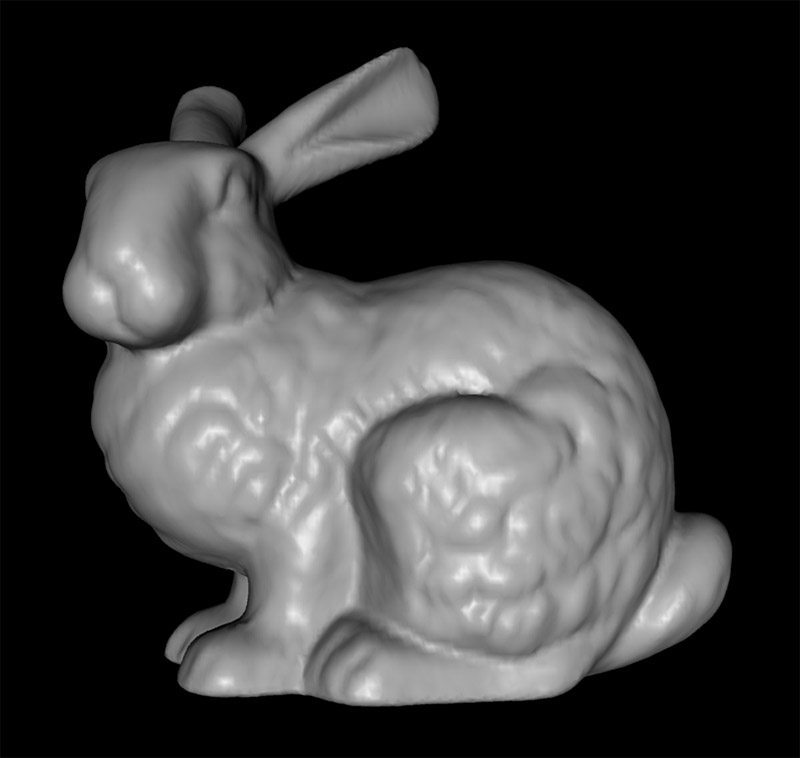
\includegraphics[
    scale=0.3
    ]{papers/sgwt/images/bunny-scanalyze-sh.jpg}
    \caption{Der Standford Bunny~\cite{noauthor_stanford_nodate} ist eines der 
    bekanntesten Testmodelle, wenn es um Computergraphiken geht.
        \label{fig:sgwt:intro:bunny}}
\end{figure}

Was ist nun aber mit Funktionen, die nicht auf einfachen K\"orperoberfl\"achen 
liegen? Zum Beispiel Funktionen auf der Oberfl\"ache des ber\"uhmten 
``Standford Bunnys''~\cite{noauthor_stanford_nodate}, zu sehen in 
\cref{fig:sgwt:intro:bunny}, welches oft als Testmodell f\"ur Computergraphiken 
eingesetzt wird. Oder bei Modellen, deren unterliegende Oberfl\"ache keine oder 
nur eine nebens\"achliche Rolle spielt, wie bei Routernetzwerken, 
Strassennetzen oder ganz generell, wenn wir nur einen Graphen haben?

In diesem Kapitel wollen wir deshalb eine Theorie entwickeln, wie 
wir die bereits bekannte Fourier- und Wavelet-Theorie auch auf einem Graphen 
anwenden 
k\"onnen, auf dessen Knoten die Funktionswerte definiert sind. Diese Theorie 
ist bekannt als ``Spectral Graph Wavelet Transform'' oder kurz SGWT -- nicht zu 
verwechseln mit der ``Second Generation Wavelet 
Transform''~\cite{noauthor_second-generation_2018}, deren K\"urzel ebenfalls 
SGWT lautet -- die erstmals 2009 in ``Wavelets on Graphs via Spectral Graph 
Theory''~\cite{hammond_wavelets_2009} vorgestellt wurde.

Wir starten mit einigen Grundlagen \"uber Graphen in~\cref{sec:sgwt:graphs} und 
gehen dann zu Laplace Operator und Matrix in~\cref{sec:sgwt:laplace} \"uber. 
Danach schauen wir uns in~\cref{sec:sgwt:spectralanalysis} die Spektralanalyse 
von Graphen genauer an und landen schlussendlich in~\cref{sec:sgwt:wavelets}, 
wo wir dann alles f\"ur die Spektral Graph Wavelet Transformation zusammen 
haben.

% !TeX spellcheck = de_CH_frami

\section{Graphen\label{sec:sgwt:graphs}}
\rhead{Graphen}

Unsere Grundlage, auf der wir die SGWT aufbauen wollen, stellen Graphen dar. 
Ein Graph $G$ setzt sich aus Kanten $E$ und Knoten $V$ zusammen.
\begin{equation*}
G = \{V, E\}
\end{equation*}
Eine Kante verbindet dabei jeweils zwei Knoten miteinander.
\begin{equation*}
E \subset \{\{v_1, v_2\} | v_i \in V, v_1 \neq v_2 \}
\end{equation*}

\begin{figure}
    \centering
    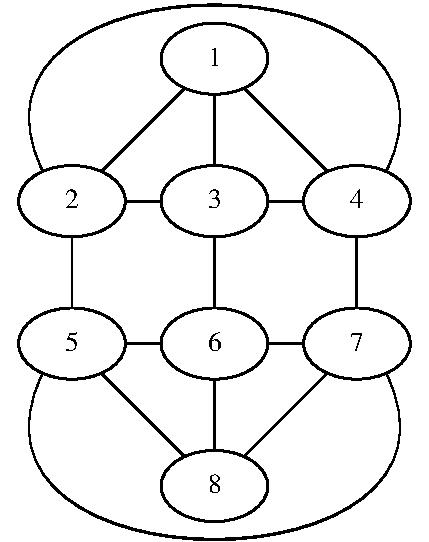
\includegraphics[
        scale=0.7
    ]{papers/sgwt/images/sphere-graph.pdf}
    \caption{Graph Approximation einer Kugel.
    \label{fig:sgwt:sphere:graph}}
\end{figure}

\begin{figure}
    \centering
    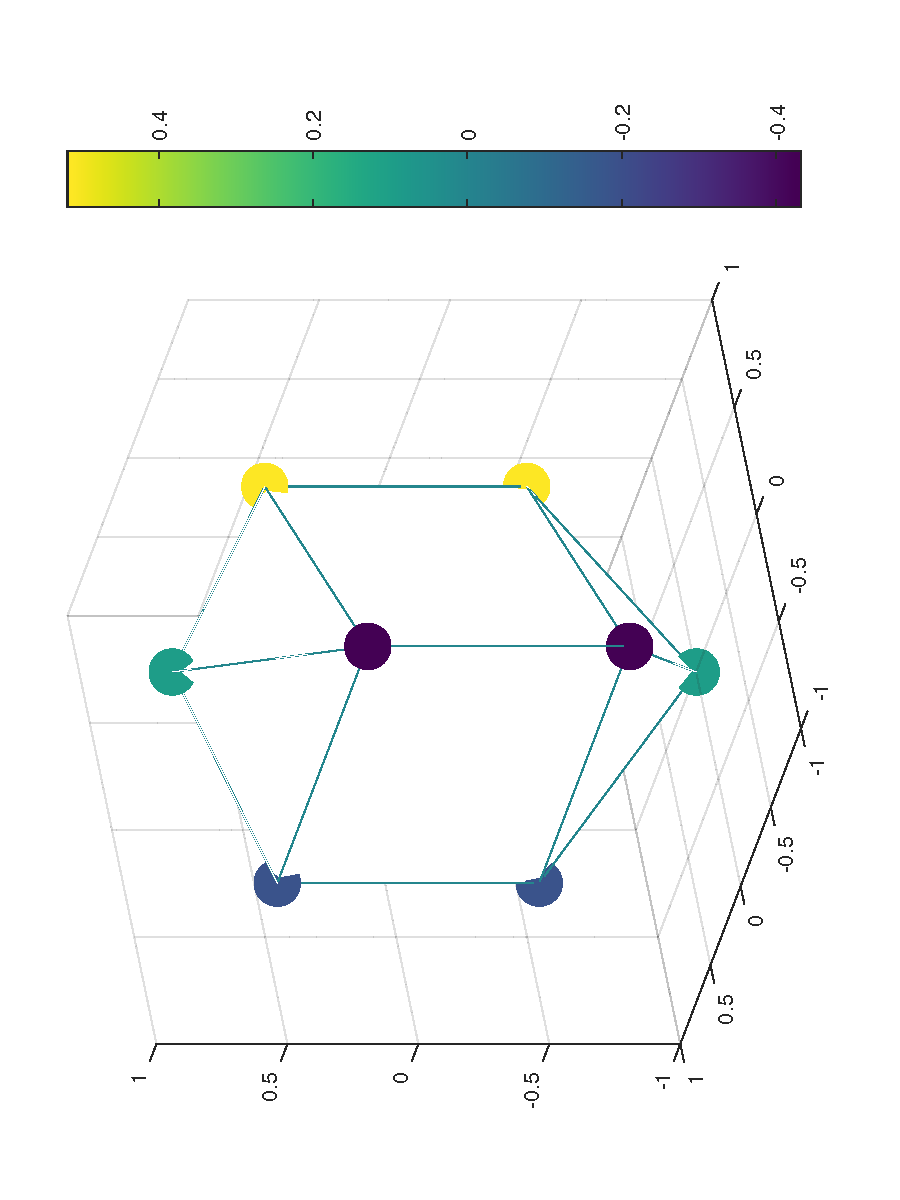
\includegraphics[
        angle=-90,
        origin=c,
        scale=0.7
    ]{papers/sgwt/images/graph-chi-4.pdf}
    \vspace{-80pt}
    \caption{Dreidimensionale Darstellung des Kugelgraphen. Die Funktionswerte 
    werden dabei mit Farben auf den Knoten dargestellt. 
    \label{fig:sgwt:sphere:graph:chi}}
\end{figure}

\begin{figure}
    \centering
    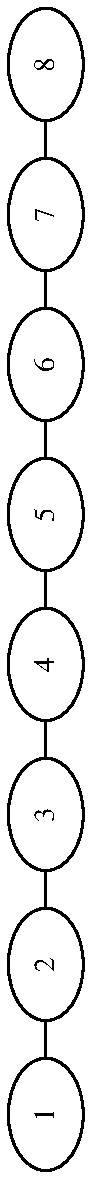
\includegraphics[
        angle=-90,
        origin=c,
        scale=0.7
    ]{papers/sgwt/images/line-graph.pdf}
    \vspace{-200pt}
    \caption{Graph Approximation einer eindimensionalen Funktion. 
    \label{fig:sgwt:line:graph}}
\end{figure}

\begin{figure}
    \centering
    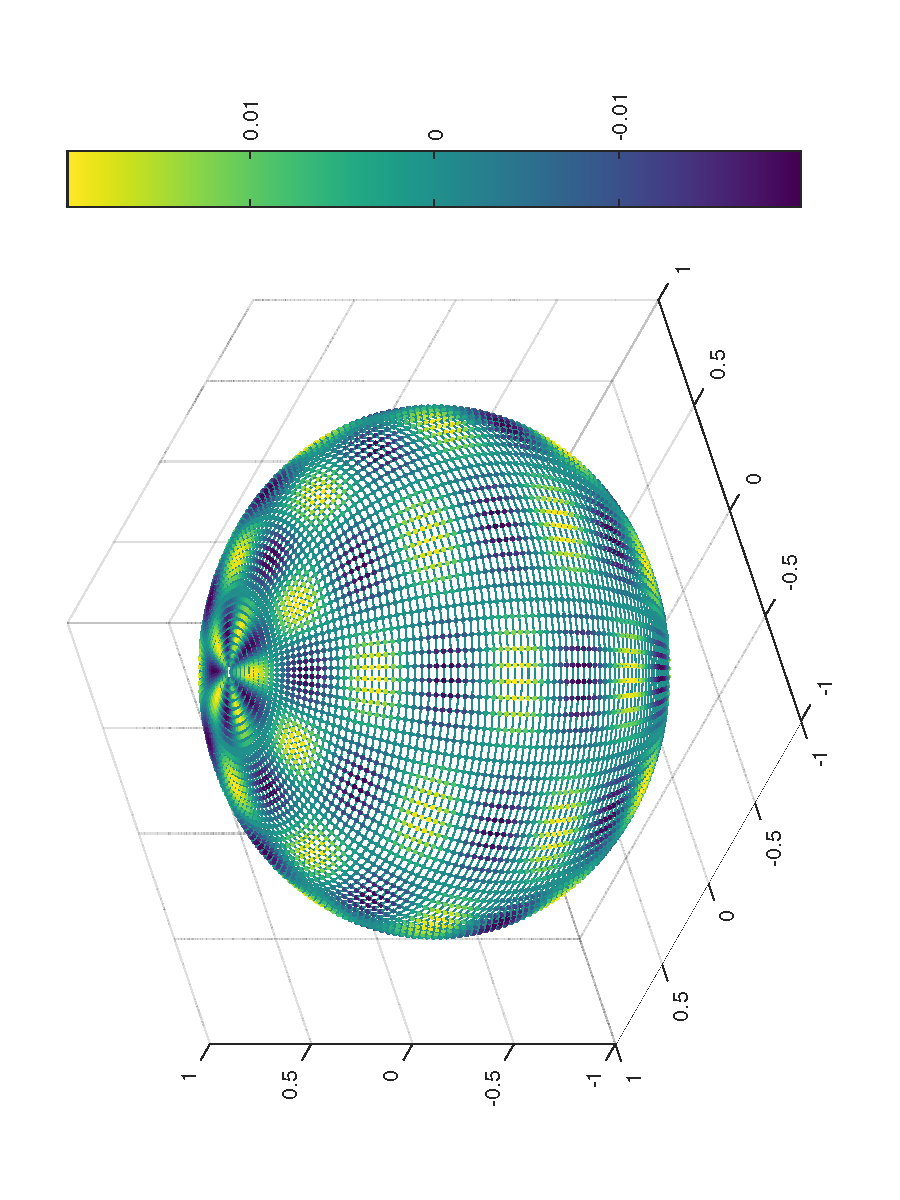
\includegraphics[
        angle=-90,
        origin=c,
        scale=0.7
    ]{papers/sgwt/images/graph-100-100-chi-150.pdf}
    \vspace{-80pt}
    \caption{Kugelgraph mit $l = b = 100$. Darstellung von $\chi_{150}$.
    \label{fig:sgwt:sphere:graph:chi:hh}}
\end{figure}

\begin{figure}
    \centering
    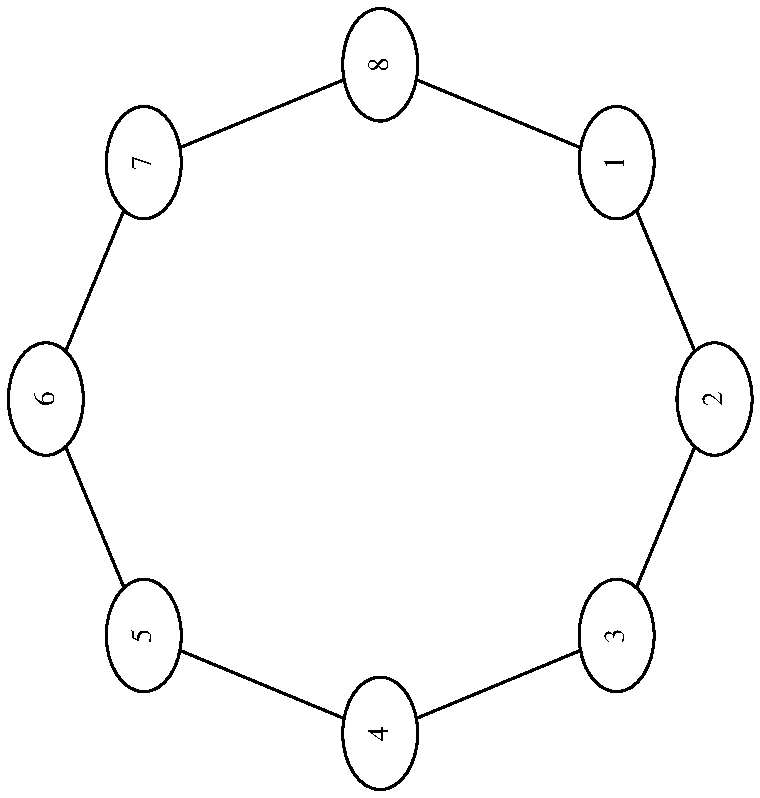
\includegraphics[
        angle=-90,
        origin=c,
        scale=0.7
    ]{papers/sgwt/images/ring-graph.pdf}
    \caption{Graph Approximation einer periodischen eindimensionalen Funktion. 
    \label{fig:sgwt:ring:graph}}
\end{figure}


\section{Laplace\label{sec:sgwt:laplace}}
\rhead{Laplace}

\subsection{Laplace Operator\label{subsec:sgwt:laplaceop}}
\rhead{Laplace Operator}

Der Laplace operator $\Delta$ in $\mathbb{R}^n$ beschreibt die zweite Ableitung.

\begin{equation}
\Delta = \frac{\partial^2}{\partial x_1^2}
+ \frac{\partial^2}{\partial x_2^2}
+ \dots
+ \frac{\partial^2}{\partial x_n^2}
\end{equation}

\subsection{Laplace Matrix\label{subsec:sgwt:laplacm}}
\rhead{Laplace Matrix}

%TODO: Why could norm be usefull?

%TODO: Rework
Die Laplace Matrix 
\laplaceL~\cite{noauthor_laplace-matrix_2017}, welche wir aus der 
Gradmatrix \degreeM~\cite{noauthor_degree_2018} und der Adjazenzmatrix 
\adjacencyM~\cite{noauthor_adjacency_2019} berechnen k\"onnen, spielt bei der 
SGWT eine entscheidende Rolle. Dabei gibt es 
die Unterscheidung zwischen der Laplace Matrix aus \cref{eq:sgwt:laplace} und 
\cref{eq:sgwt:laplace:norm}, bei der \laplaceLnorm{} Matrix handelt es sich um 
die normalisierte \laplaceL{} Matrix.

\begin{equation}
\laplaceL = \degreeM - \adjacencyM
\label{eq:sgwt:laplace}
\end{equation}

\begin{equation}
\laplaceLnorm
= \degreeM^{-1/2}\laplaceL\degreeM^{-1/2}
= I - \degreeM^{-1/2}\adjacencyM\degreeM^{-1/2}
\label{eq:sgwt:laplace:norm}
\end{equation}

\begin{equation}
\chi = 
\left[
\begin{pmatrix}\\\chi_0\\\\\end{pmatrix}
\begin{pmatrix}\\\chi_1\\\\\end{pmatrix}
\begin{pmatrix}\\\chi_2\\\\\end{pmatrix}
\cdots
\begin{pmatrix}\\\chi_{N-1}\\\\\end{pmatrix}
\right]
\end{equation}

\begin{equation}
0 = \lambda_0 < \lambda_1 \le \lambda_2 \le \cdots \le \lambda_{N-1}
\end{equation}

% !TeX spellcheck = de_CH_frami

\section{Graph Spektralanalyse\label{sec:sgwt:spectralanalysis}}
\rhead{Graph Spektralanalyse}

Nachdem wir nun die Grundlagen von Graphen und den Laplace Operator sowie die 
Laplace Matrix angeschaut haben, wollen wir uns nun der Spektralanalyse eines 
Graphen widmen.

\subsection{Laplace Matrix Eigenwerte}

Wenn man vom Spektrum eines Graphen spricht, meint man damit die Eigenwerte 
$\lambda$ seiner Laplace Matrix. Da diese Matrix bei einem ungerichteten 
Graphen immer symmetrisch ist, werden die daraus folgenden Eigenwerte und 
Eigenfunktionen auch immer real und gr\"osser gleich $0$ sein. Es gilt somit
\begin{equation}
0 = \lambda_0 < \lambda_1 \leq \lambda_2 \leq \cdots \leq \lambda_{N-1}.
\label{eq:sgwt:lambda:series}
\end{equation}
\Cref{fig:sgwt:lambda:line} zeigt die Eigenwerte $\lambda_0$ bis 
$\lambda_{999}$ eines Ringraphen mit 1000 Knoten.

\begin{figure}
    \centering
    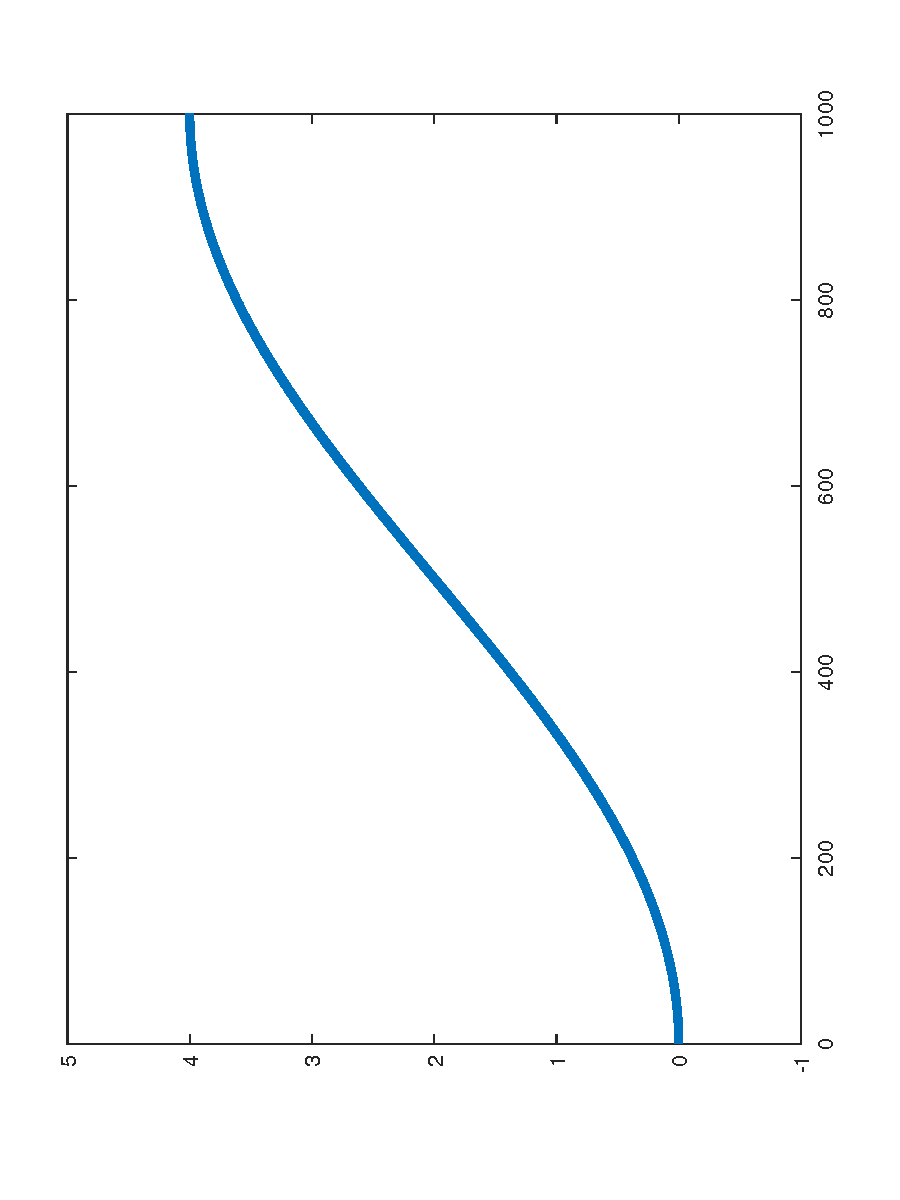
\includegraphics[
    angle=-90,
    origin=c,
    scale=0.6
    ]{papers/sgwt/images/ring-lambda.pdf}
    \vspace{-70pt}
    \caption{$\lambda_0$ bis $\lambda_{999}$ eines nicht gewichteten Ringraphen.
        \label{fig:sgwt:lambda:line}}
\end{figure}

\subsection{Laplace Matrix Eigenvektoren}

Eine weitere wichtige Rolle spielen die Eigenvektoren der Laplace Matrix. Diese 
sind n\"amlich approximierte Eigenfunktionen des Laplace Operators $\Delta$. So 
ist die komplexe Exponentialfunktion $e^{i\omega x}$ die Eigenfunktion des 
eindimensionalen Laplace Operators 
$\frac{d^2}{dx^2}$~\cite{chung_spectral_nodate}. Dies wird deutlich, wenn 
wir die Eigenfunktionen eines 
Ring-,~\cref{fig:sgwt:chi:ring0,fig:sgwt:chi:ring1,fig:sgwt:chi:ring2,fig:sgwt:chi:ring3,fig:sgwt:chi:ring4,fig:sgwt:chi:ring5},
oder 
Liniengraphen,~\cref{fig:sgwt:chi:line0,fig:sgwt:chi:line1,fig:sgwt:chi:line2,fig:sgwt:chi:line3,fig:sgwt:chi:line4,fig:sgwt:chi:line5},
darstellen. Auch die Kugelfunktionen $Y^m_l$, lassen mit den Hilfe der 
Eigenfunktionen eines Kugelgraphen approximieren, wie man 
in~\cref{fig:sgwt:chi:sphere} sehen kann. Dabei wird aber auch deutlich, dass 
diese Approximation nicht \"uberall gleich gut ist. Insbesondere dadurch, dass 
der Grad an den Polen stark von den anderen Knoten abweicht, findet dort eine 
Verzerrung statt.

\begin{figure}
\centering
\begin{minipage}[b]{0.49\textwidth}
    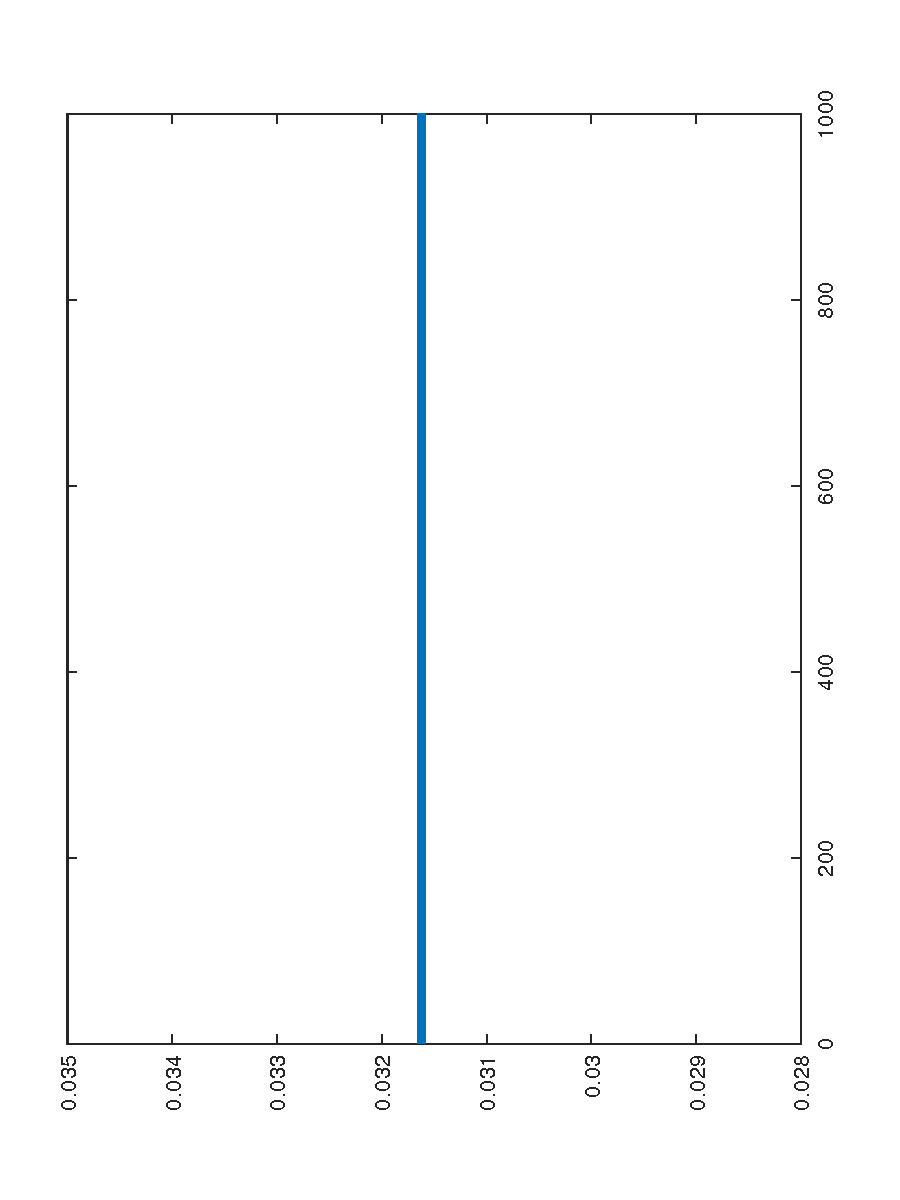
\includegraphics[
    angle=-90,
    origin=c,
    width=\textwidth]{papers/sgwt/images/ring-chi-1.pdf}
    \vspace{-45pt}
    \caption{$\chi_0$ eines ungewichteten Ringraphen mit 1000 Knoten.}
    \label{fig:sgwt:chi:ring0}
\end{minipage}
~
\begin{minipage}[b]{0.49\textwidth}
    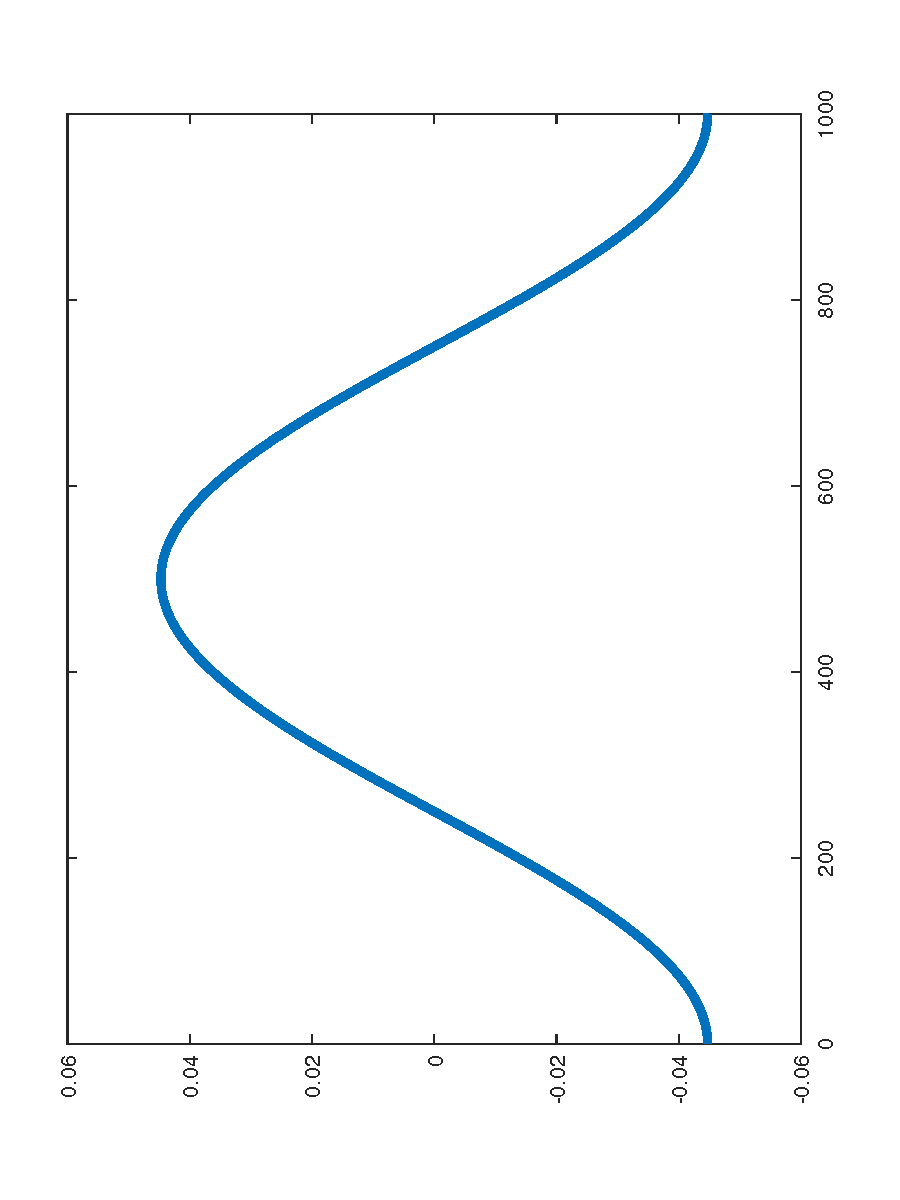
\includegraphics[
    angle=-90,
    origin=c,
    width=\textwidth]{papers/sgwt/images/ring-chi-2.pdf}
    \vspace{-45pt}
    \caption{$\chi_1$ eines ungewichteten Ringraphen mit 1000 Knoten.}
    \label{fig:sgwt:chi:ring1}
\end{minipage}
~
\begin{minipage}[b]{0.49\textwidth}
    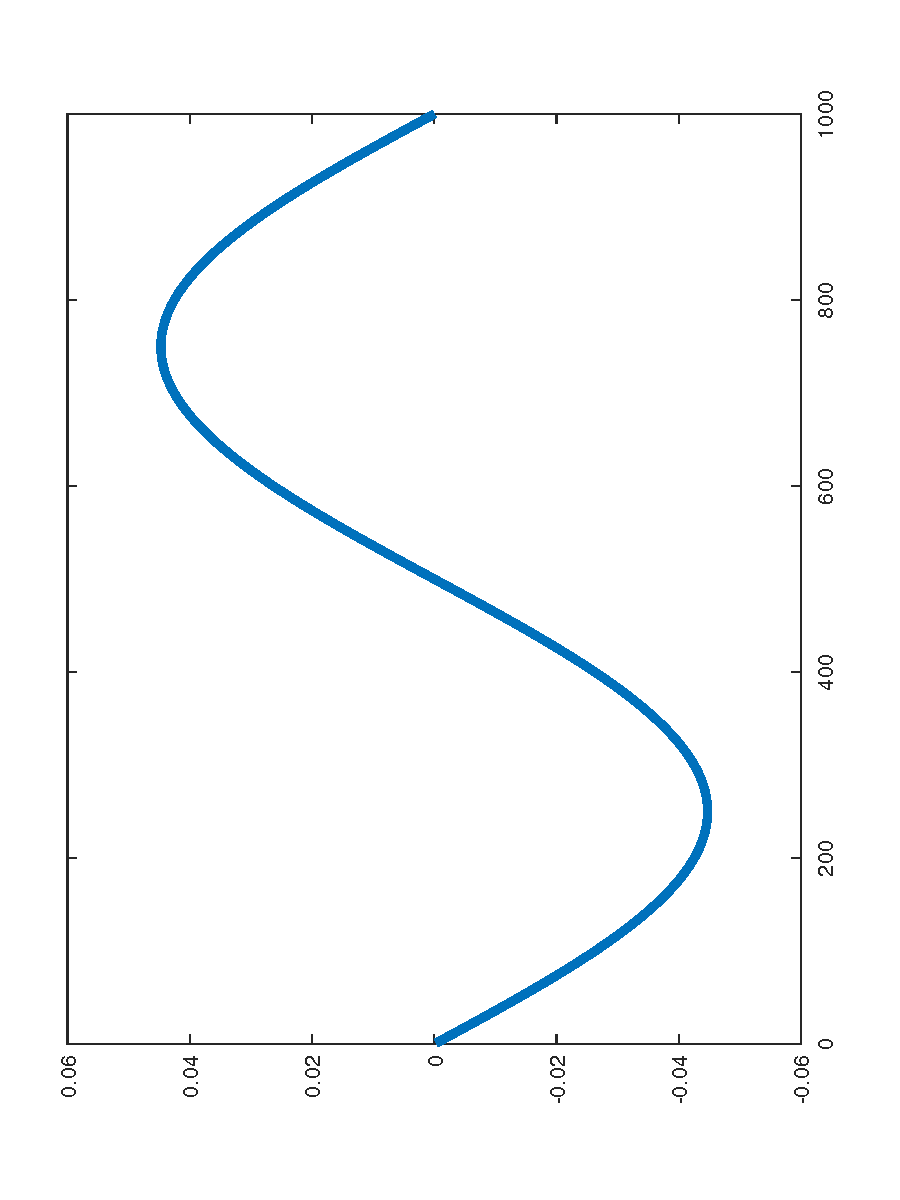
\includegraphics[
    angle=-90,
    origin=c,
    width=\textwidth]{papers/sgwt/images/ring-chi-3.pdf}
    \vspace{-45pt}
    \caption{$\chi_2$ eines ungewichteten Ringraphen mit 1000 Knoten.}
    \label{fig:sgwt:chi:ring2}
\end{minipage}
~
\begin{minipage}[b]{0.49\textwidth}
    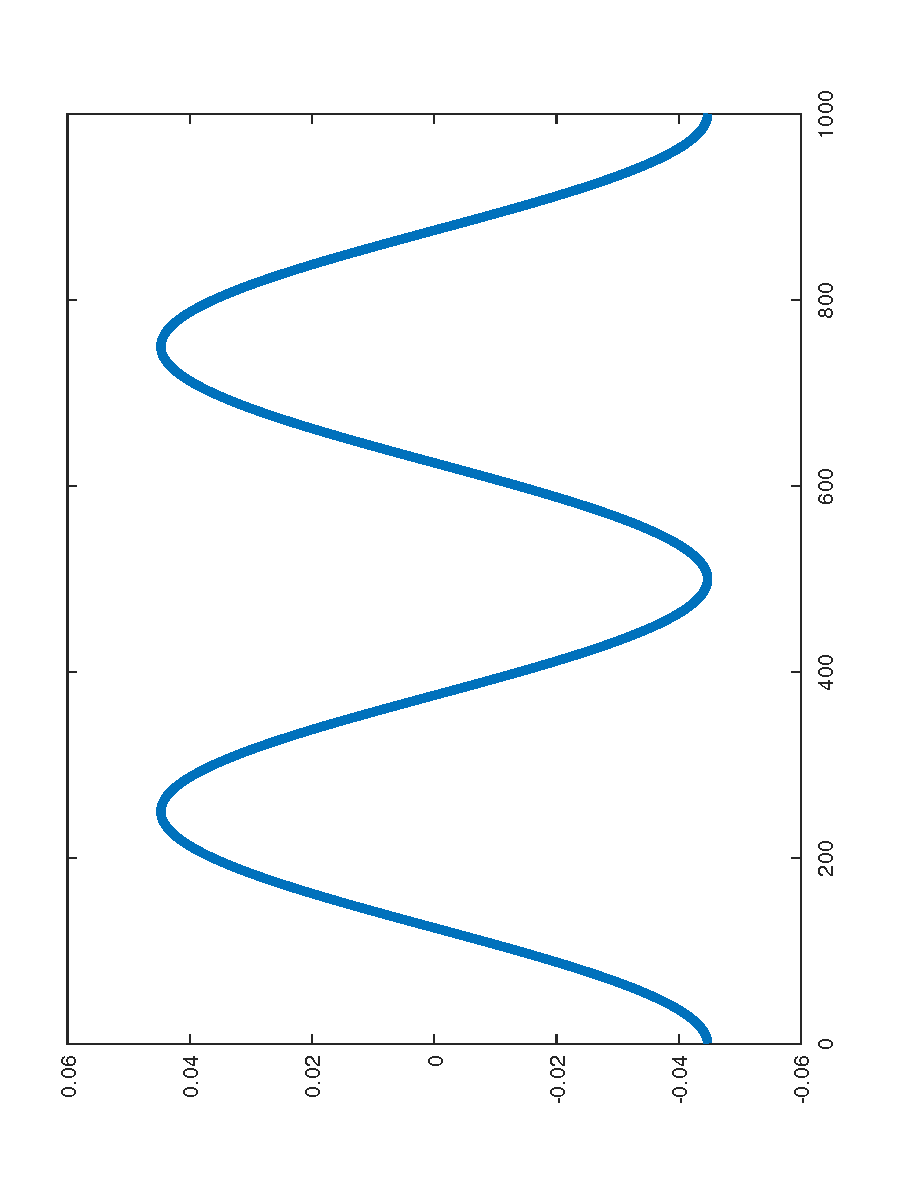
\includegraphics[
    angle=-90,
    origin=c,
    width=\textwidth]{papers/sgwt/images/ring-chi-4.pdf}
    \vspace{-45pt}
    \caption{$\chi_3$ eines ungewichteten Ringraphen mit 1000 Knoten.}
    \label{fig:sgwt:chi:ring3}
\end{minipage}
~
\begin{minipage}[b]{0.49\textwidth}
    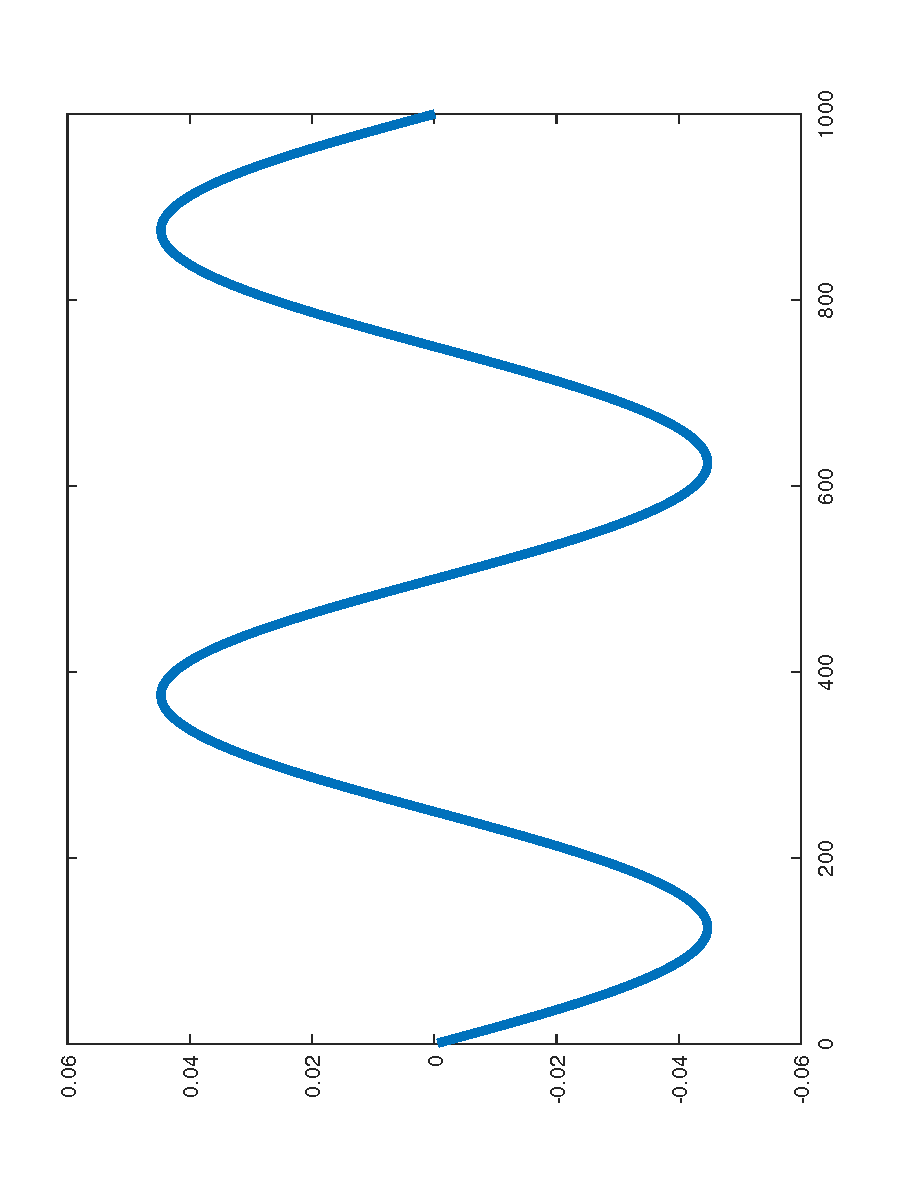
\includegraphics[
    angle=-90,
    origin=c,
    width=\textwidth]{papers/sgwt/images/ring-chi-5.pdf}
    \vspace{-45pt}
    \caption{$\chi_4$ eines ungewichteten Ringraphen mit 1000 Knoten.}
    \label{fig:sgwt:chi:ring4}
\end{minipage}
~
\begin{minipage}[b]{0.49\textwidth}
    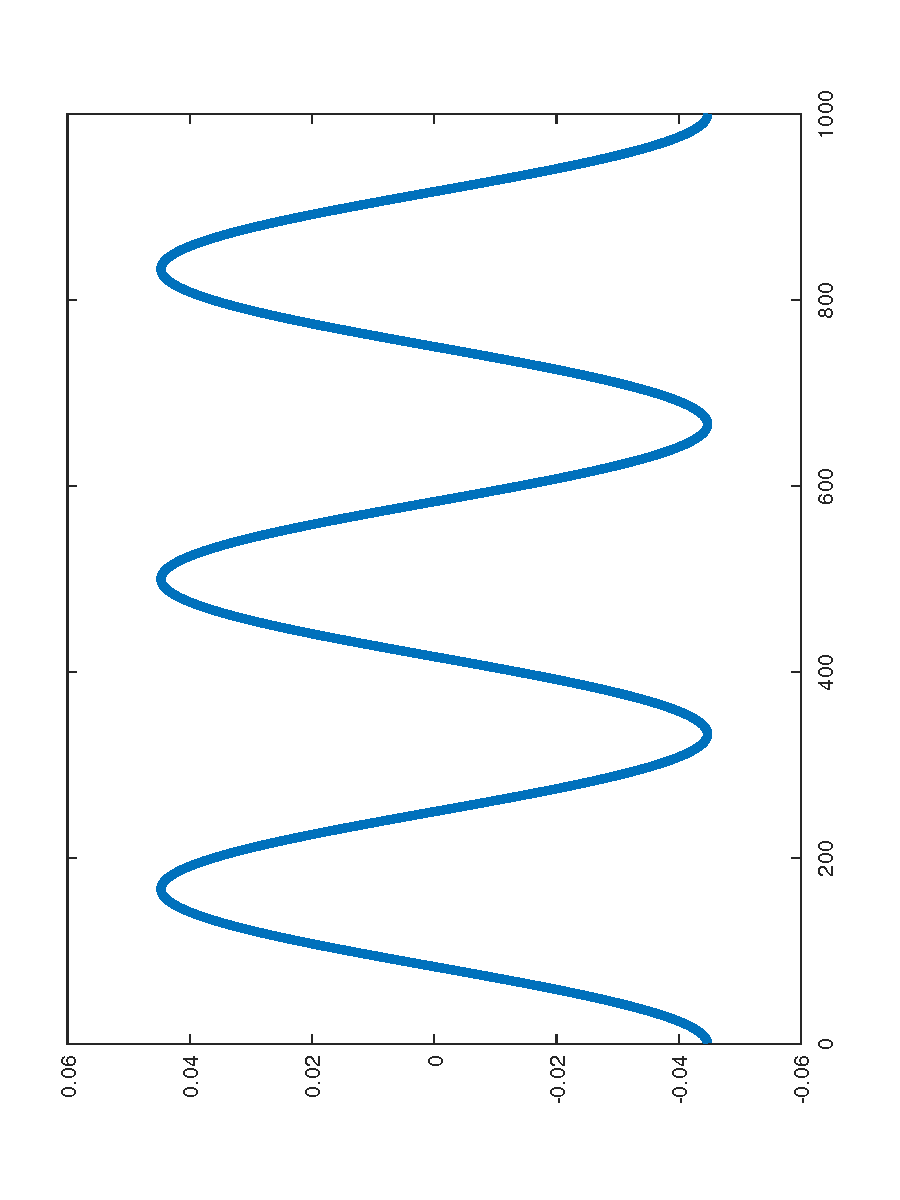
\includegraphics[
    angle=-90,
    origin=c,
    width=\textwidth]{papers/sgwt/images/ring-chi-6.pdf}
    \vspace{-45pt}
    \caption{$\chi_5$ eines ungewichteten Ringraphen mit 1000 Knoten.}
    \label{fig:sgwt:chi:ring5}
\end{minipage}
\end{figure}

\begin{figure}
    \centering
    \begin{minipage}[b]{0.49\textwidth}
        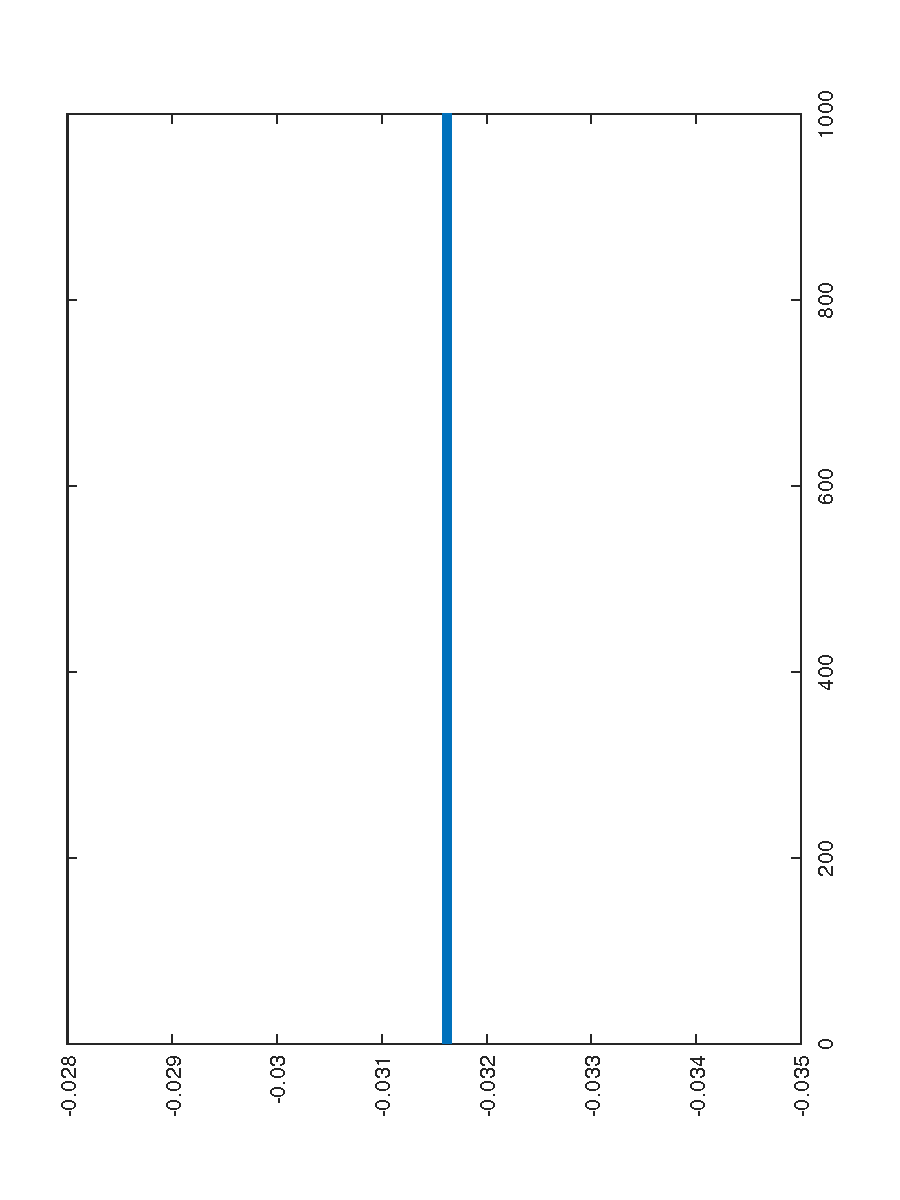
\includegraphics[
        angle=-90,
        origin=c,
        width=\textwidth]{papers/sgwt/images/line-chi-1.pdf}
        \vspace{-45pt}
        \caption{$\chi_0$ eines ungewichteten Liniengraphen mit 1000 
        Knoten.}
        \label{fig:sgwt:chi:line0}
    \end{minipage}
    ~
    \begin{minipage}[b]{0.49\textwidth}
        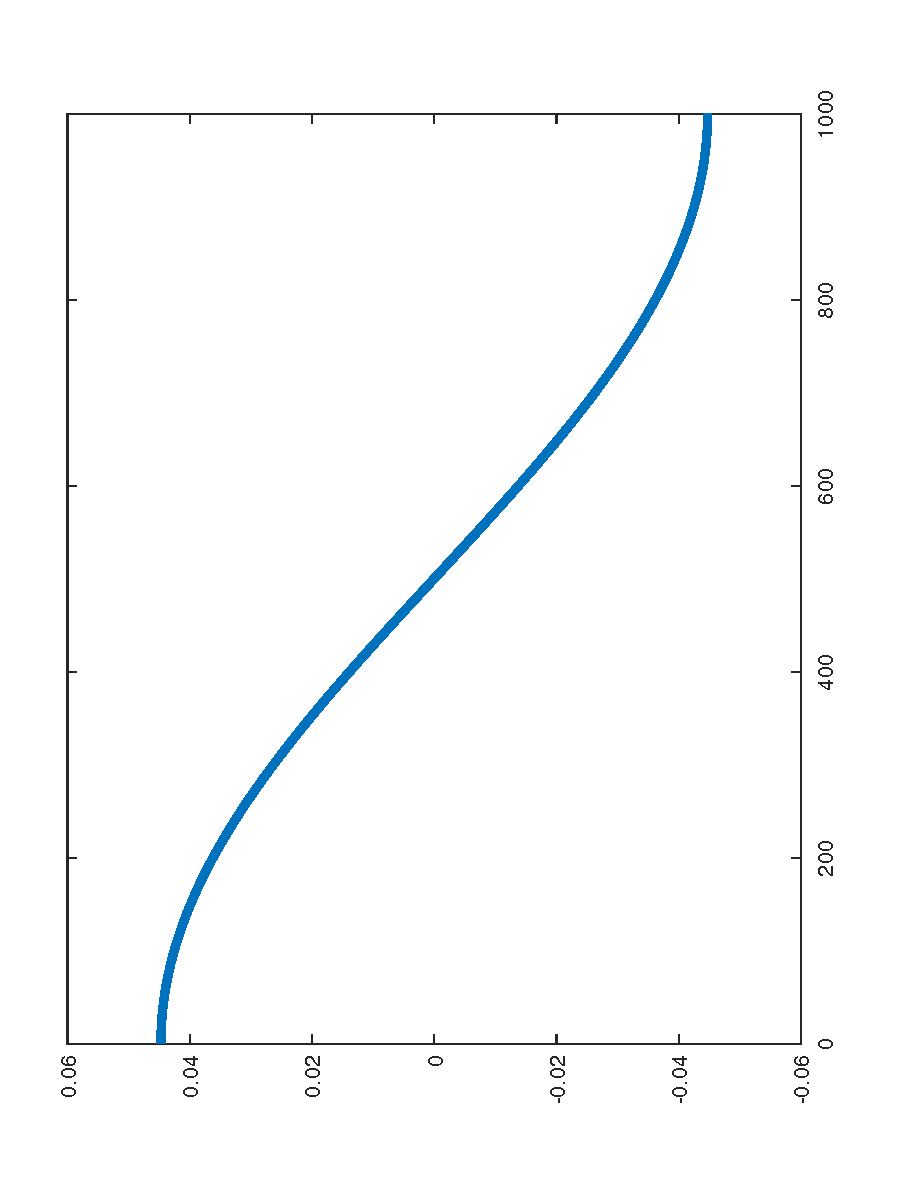
\includegraphics[
        angle=-90,
        origin=c,
        width=\textwidth]{papers/sgwt/images/line-chi-2.pdf}
        \vspace{-45pt}
        \caption{$\chi_1$ eines ungewichteten Liniengraphen mit 1000 
        Knoten.}
        \label{fig:sgwt:chi:line1}
    \end{minipage}
    ~
    \begin{minipage}[b]{0.49\textwidth}
        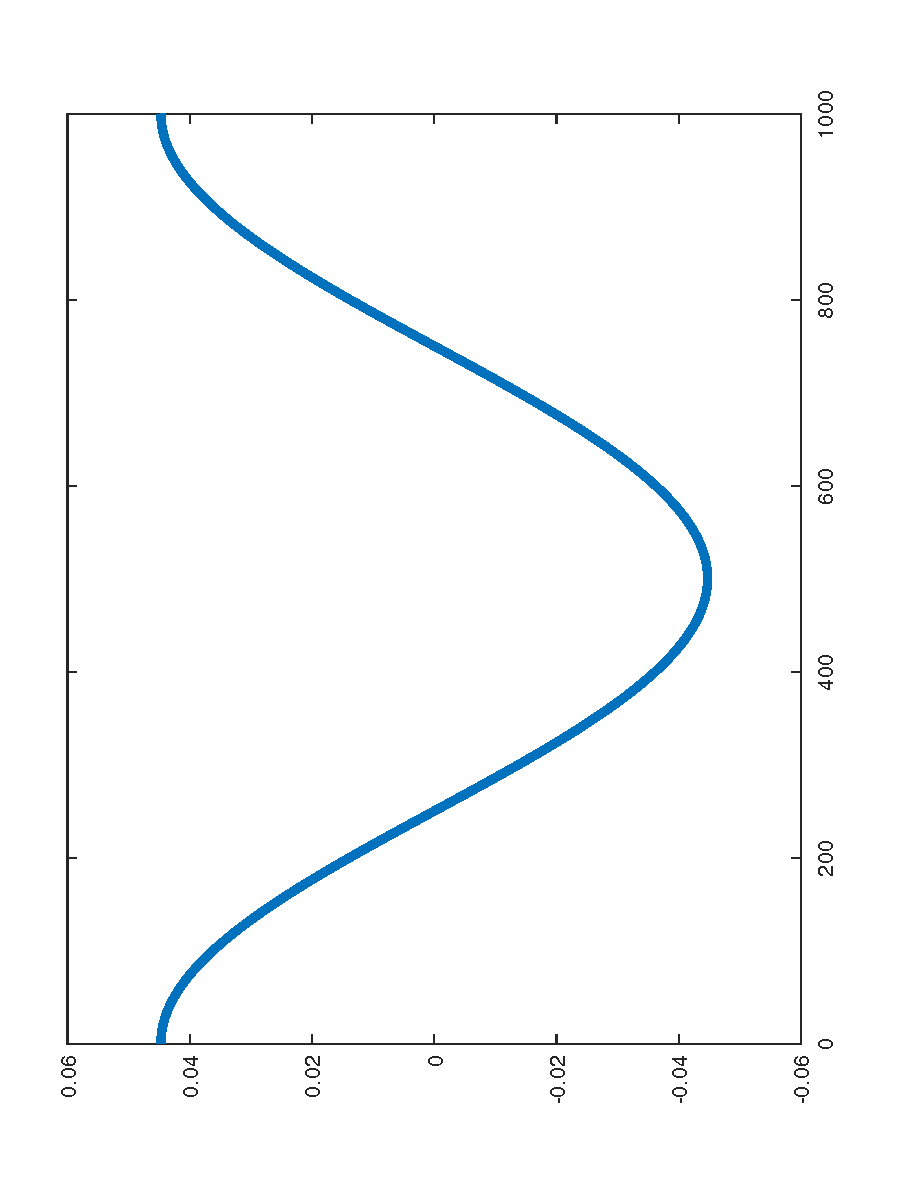
\includegraphics[
        angle=-90,
        origin=c,
        width=\textwidth]{papers/sgwt/images/line-chi-3.pdf}
        \vspace{-45pt}
        \caption{$\chi_2$ eines ungewichteten Liniengraphen mit 1000 
        Knoten.}
        \label{fig:sgwt:chi:line2}
    \end{minipage}
    ~
    \begin{minipage}[b]{0.49\textwidth}
        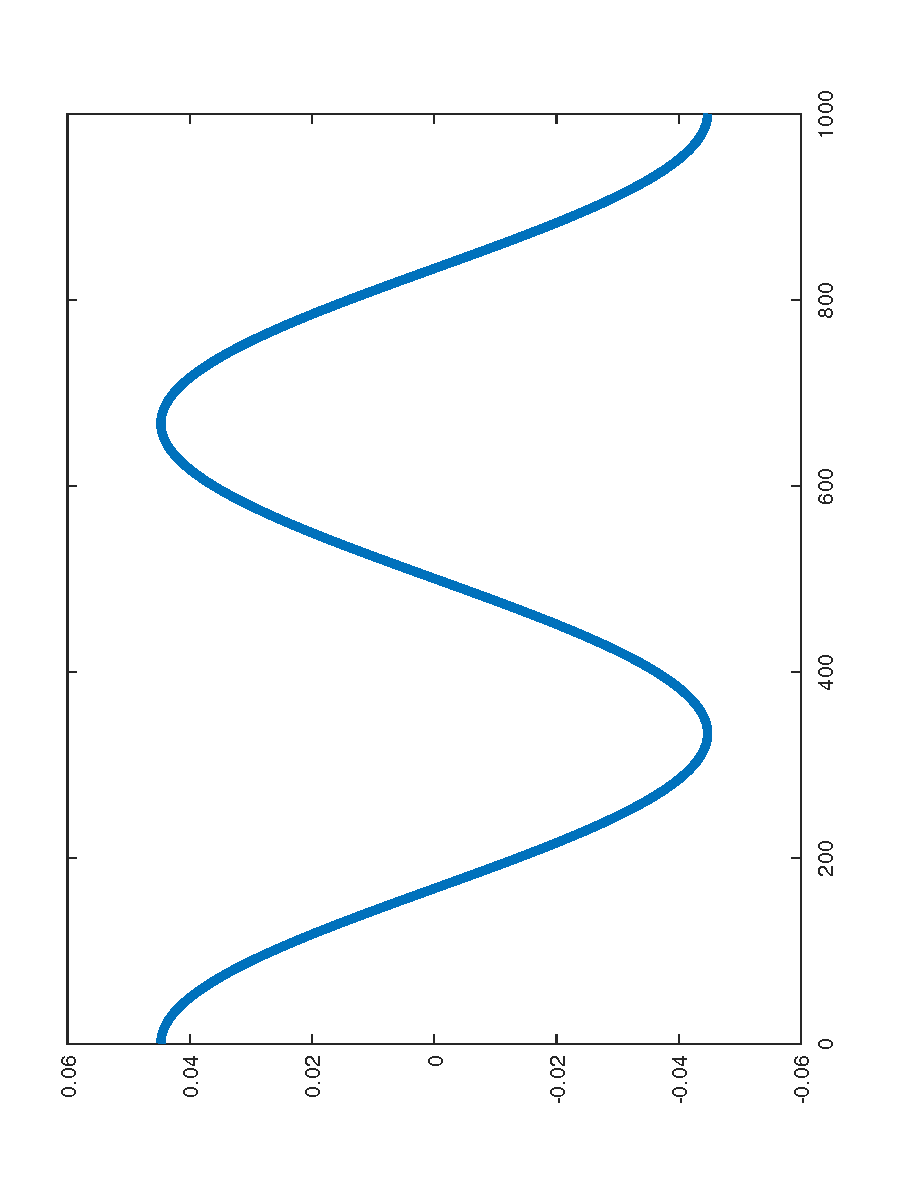
\includegraphics[
        angle=-90,
        origin=c,
        width=\textwidth]{papers/sgwt/images/line-chi-4.pdf}
        \vspace{-45pt}
        \caption{$\chi_3$ eines ungewichteten Liniengraphen mit 1000 
        Knoten.}
        \label{fig:sgwt:chi:line3}
    \end{minipage}
    ~
    \begin{minipage}[b]{0.49\textwidth}
        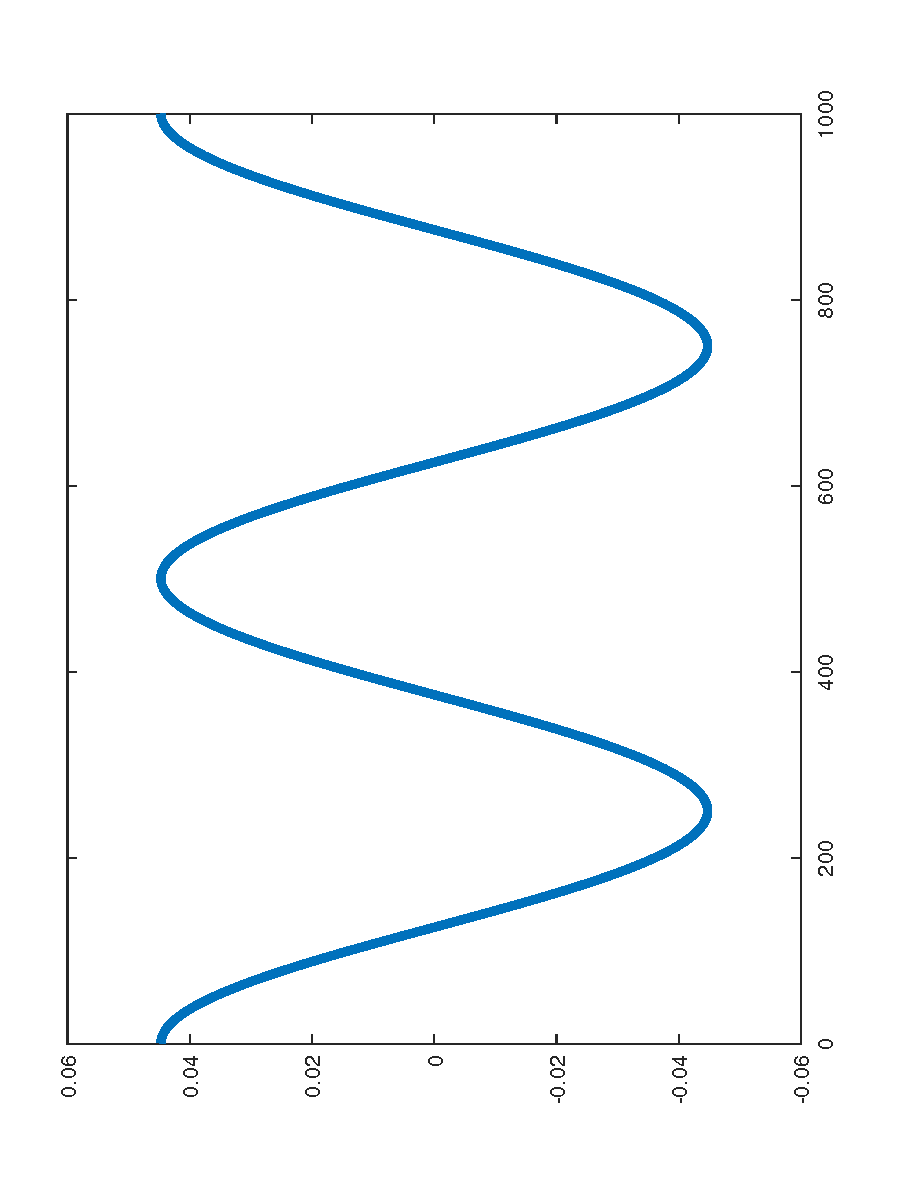
\includegraphics[
        angle=-90,
        origin=c,
        width=\textwidth]{papers/sgwt/images/line-chi-5.pdf}
        \vspace{-45pt}
        \caption{$\chi_4$ eines ungewichteten Liniengraphen mit 1000 
        Knoten.}
        \label{fig:sgwt:chi:line4}
    \end{minipage}
    ~
    \begin{minipage}[b]{0.49\textwidth}
        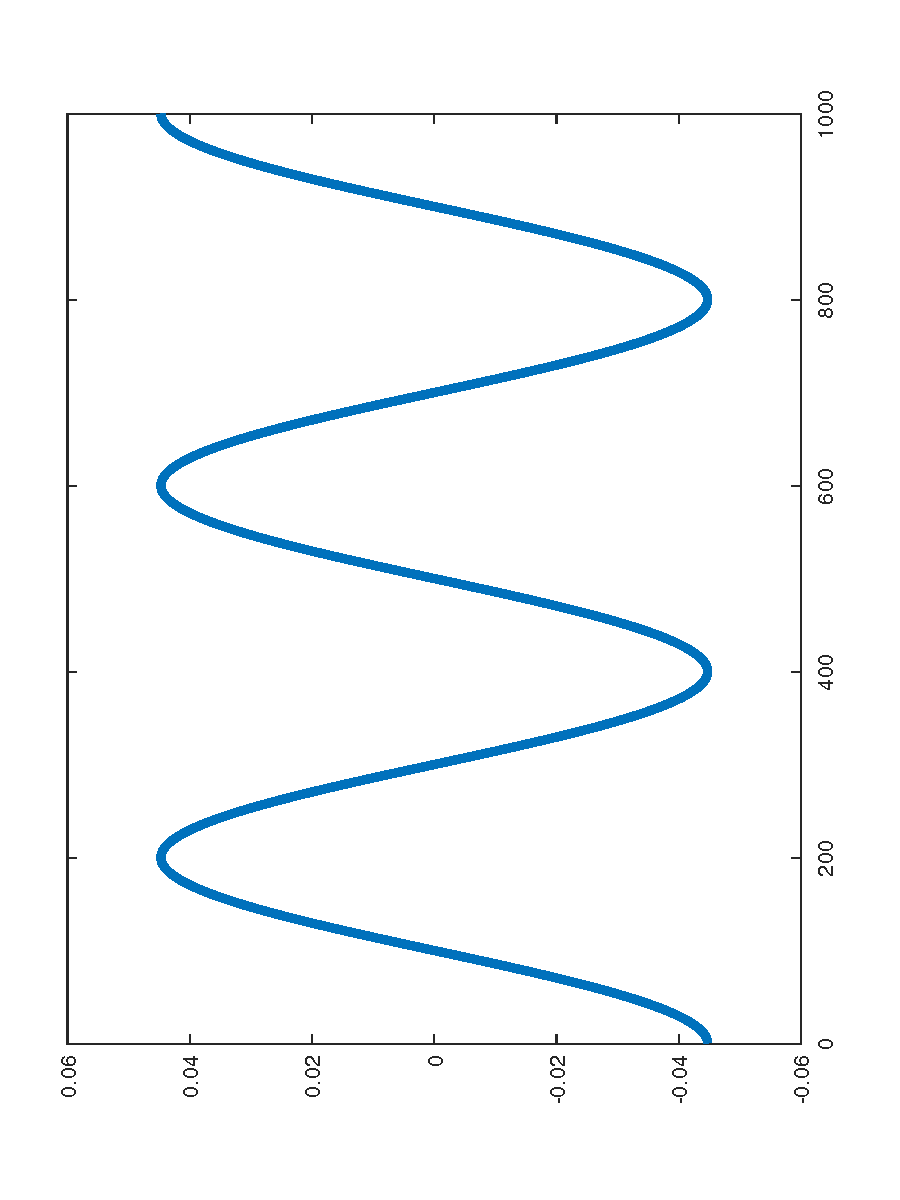
\includegraphics[
        angle=-90,
        origin=c,
        width=\textwidth]{papers/sgwt/images/line-chi-6.pdf}
        \vspace{-45pt}
        \caption{$\chi_5$ eines ungewichteten Liniengraphen mit 1000 
        Knoten.}
        \label{fig:sgwt:chi:line5}
    \end{minipage}
\end{figure}

\begin{figure}
    \centering
    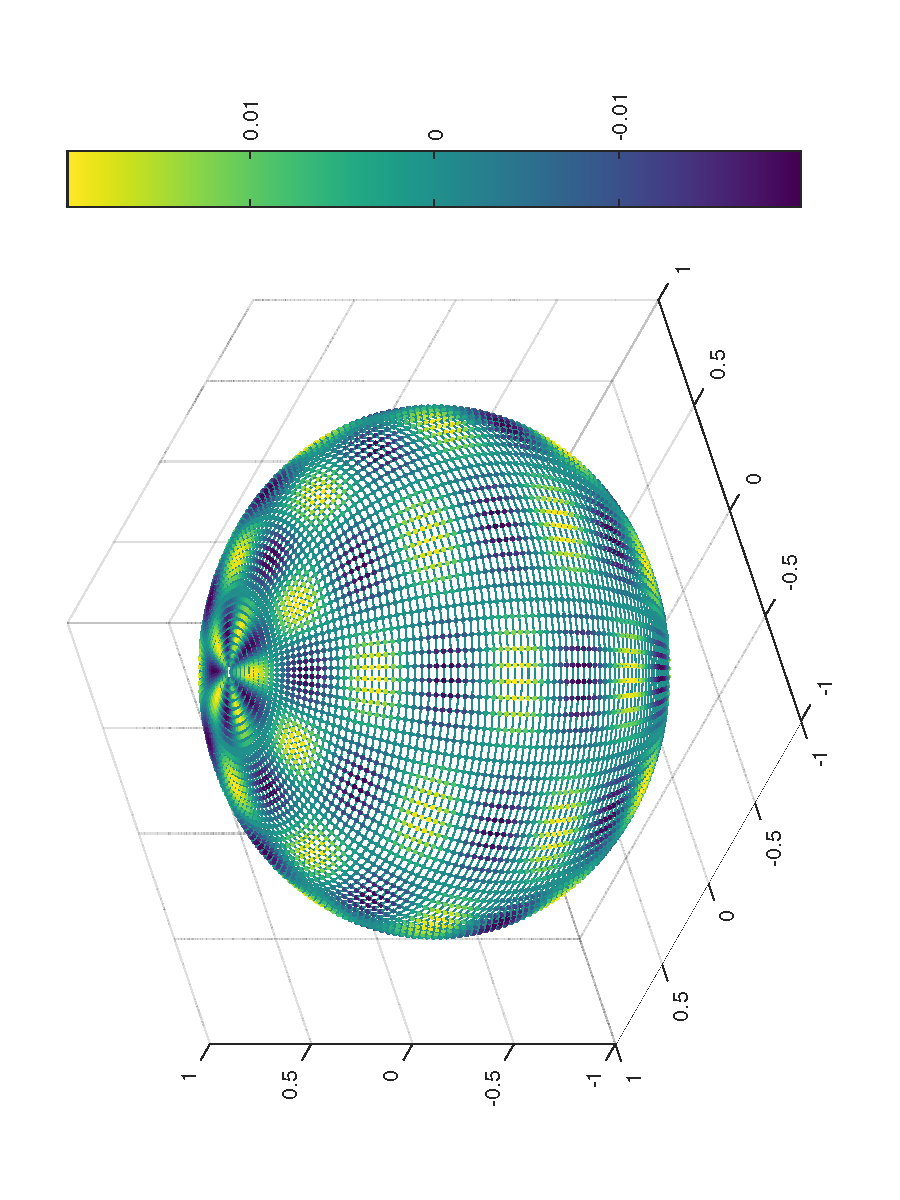
\includegraphics[
    angle=-90,
    origin=c,
    scale=0.7
    ]{papers/sgwt/images/graph-100-100-chi-150.pdf}
    \vspace{-80pt}
    \caption{Kugelgraph mit 10002 Knoten. Darstellung von $\chi_{150}$.
        \label{fig:sgwt:chi:sphere}}
\end{figure}
% !TeX spellcheck = de_CH_frami

\section{Spectral Graph Wavelet Transformation\label{sec:sgwt:wavelets}}
\rhead{SGWT}

Hier wollen wir nun das Bisherige zur Spectral Graph Wavelet Transformation 
vereinen.

\subsection{Graph Fourier Transformation\label{subsec:sgwt:gft}}

Bevor wir uns auf die Graph Wavelets st\"urzen, wollen wir zuerst versuchen die 
Fourier Theorie auf Funktionen auf Graphen anzuwenden. Dazu nehmen wir das 
Beispiel eines Dirac-Stosses $\delta(x)$, siehe~\cref{fig:sgwt:gft:dirac}.
\begin{figure}
    \centering
    \begin{minipage}[b]{0.49\textwidth}
    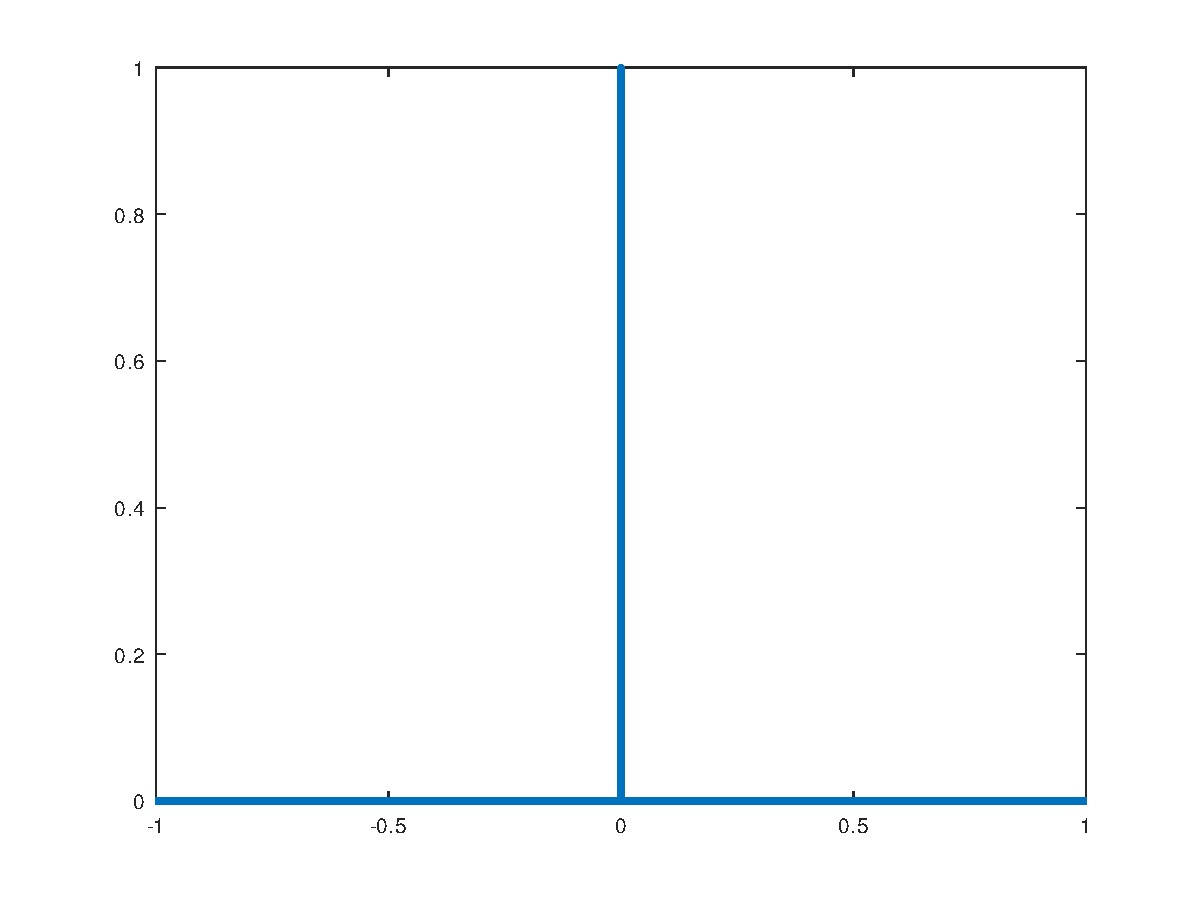
\includegraphics[
    width=\textwidth
    ]{papers/sgwt/images/dirac/dirac_delta.pdf}
    \vspace{-0pt}
    \caption{Darstellung eines Dirac-Stoss $\delta(x)$ mit maximal Wert $1$. 
        \label{fig:sgwt:gft:dirac}}
    \end{minipage}
    ~
    \begin{minipage}[b]{0.49\textwidth}
    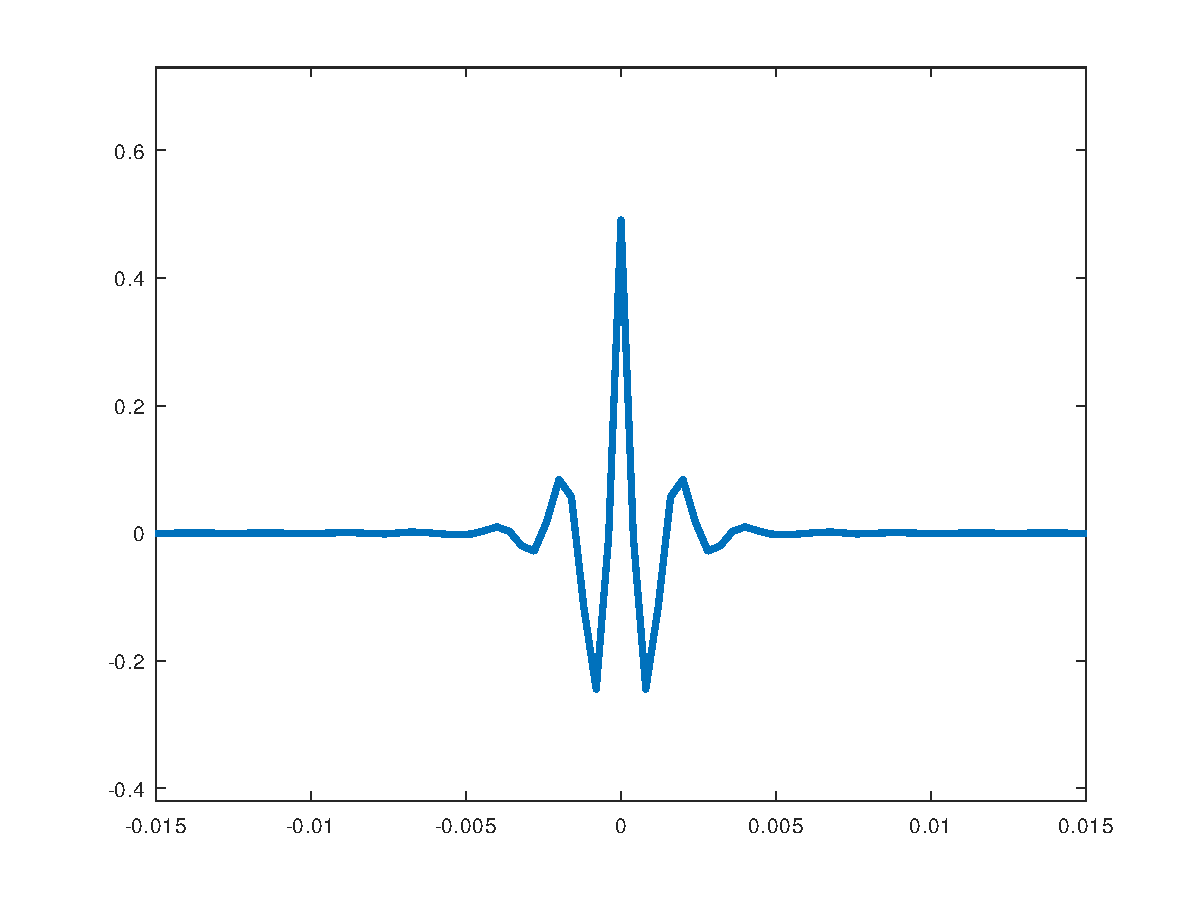
\includegraphics[
    width=\textwidth
    ]{papers/sgwt/images/dirac/dirac_g_igft.pdf}
    \vspace{-0pt}
    \caption{Fourier Transformation des Dirac-Stosses $\hat{\delta(x)}$ 
        aus~\cref{fig:sgwt:gft:dirac}.\label{fig:sgwt:gft:igft}}
    \end{minipage}
    ~
    \begin{minipage}[b]{0.49\textwidth}
    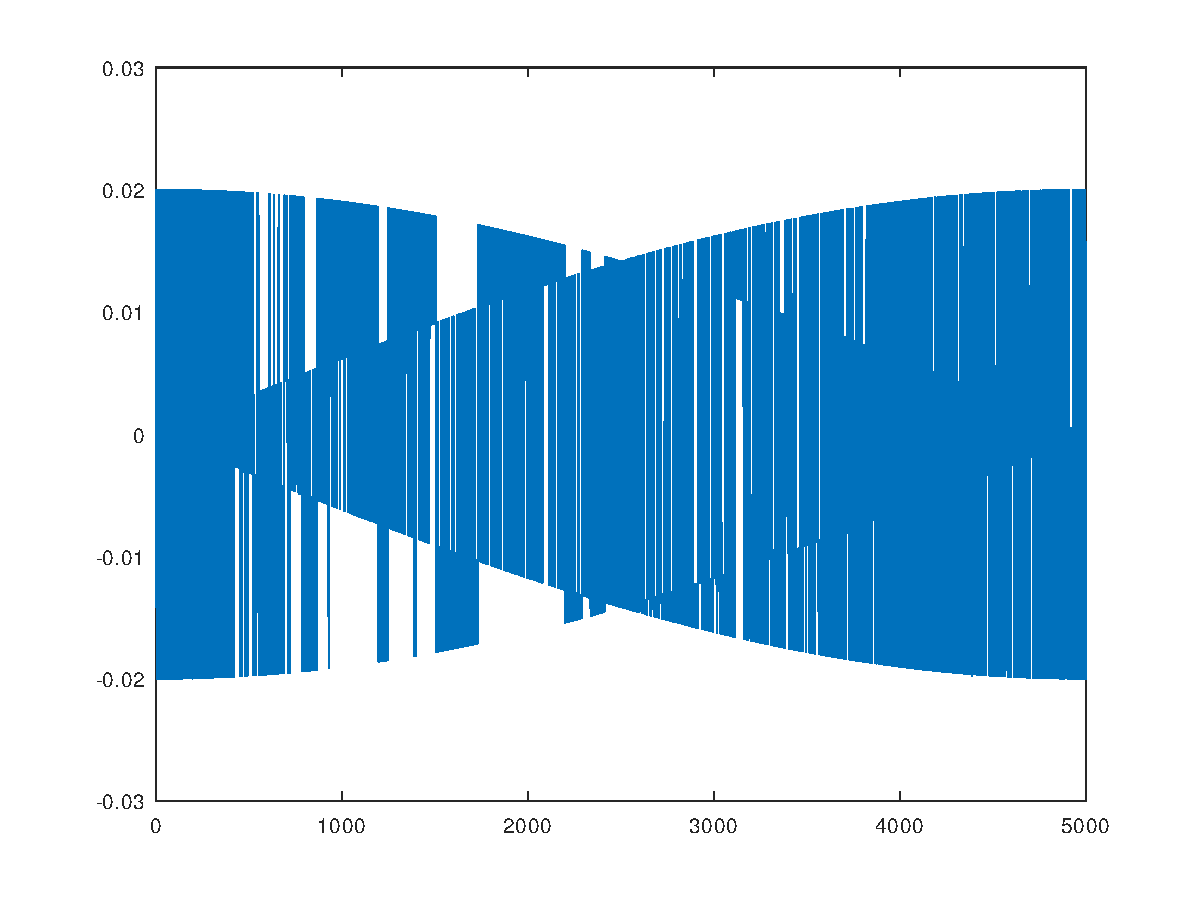
\includegraphics[
    width=\textwidth
    ]{papers/sgwt/images/dirac/dirac_gft.pdf}
    \vspace{-0pt}
    \caption{Fourier Transformation des Dirac-Stosses $\hat{\delta(x)}$ 
        aus~\cref{fig:sgwt:gft:dirac}.\label{fig:sgwt:gft:gft}}
    \end{minipage}
    ~
    \begin{minipage}[b]{0.49\textwidth}
    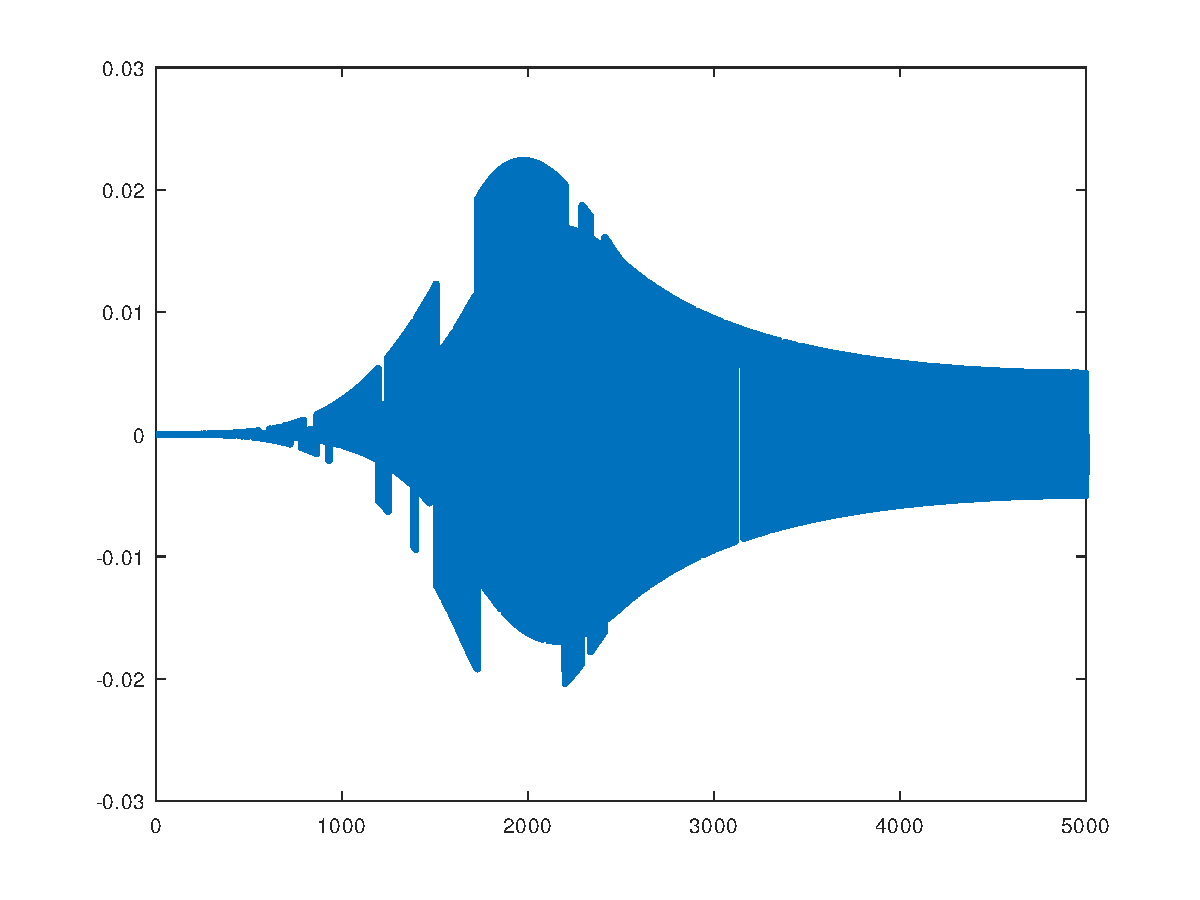
\includegraphics[
    width=\textwidth
    ]{papers/sgwt/images/dirac/dirac_g_gft.pdf}
    \vspace{-0pt}
    \caption{Fourier Transformation des Dirac-Stosses $\hat{\delta(x)}$ 
        aus~\cref{fig:sgwt:gft:dirac}.\label{fig:sgwt:gft:ggft}}
    \end{minipage}
\end{figure}
Wenn wir davon die Fourier Transformation berechnen, zu sehen 
in~\cref{fig:sgwt:gft:fftdirac}, stellen wir fest, das nicht nur alle 
Frequenzen vorhanden sondern auch alle gleich stark vorhanden sind. Die 
Fouriertransformierte $\hat{\delta}$ ist somit vollst\"andig delokalisiert.

$g(\lambda)\cdot\hat{\delta}(\lambda)$

\begin{figure}
    \centering
    \begin{minipage}[b]{0.49\textwidth}
    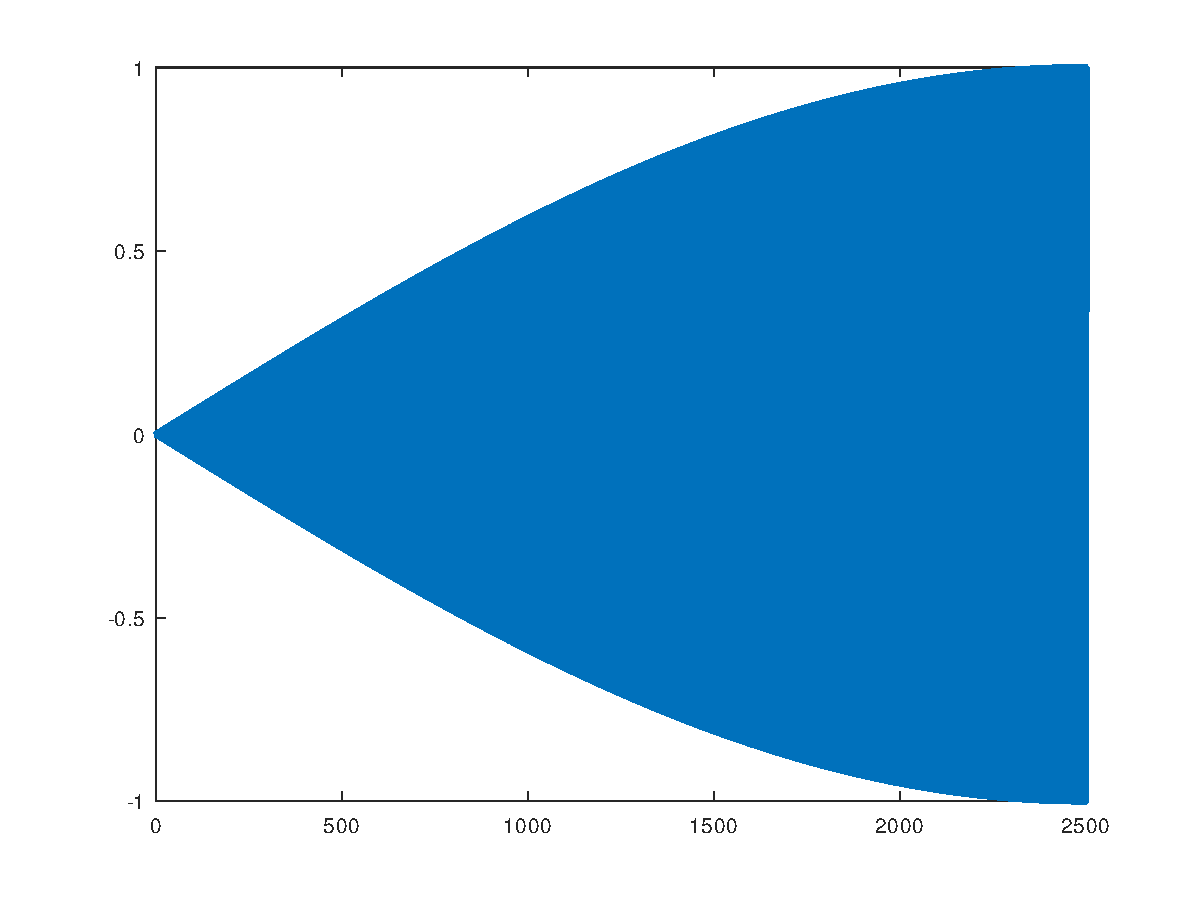
\includegraphics[
    width=\textwidth
    ]{papers/sgwt/images/dirac/dirac_fft_imag.pdf}
    \vspace{-0pt}
    \caption{Darstellung eines Dirac-Stoss $\delta(x)$ mit maximal Wert $1$. 
        \label{fig:sgwt:gft:dirac}}
    \end{minipage}
    ~
    \begin{minipage}[b]{0.49\textwidth}
    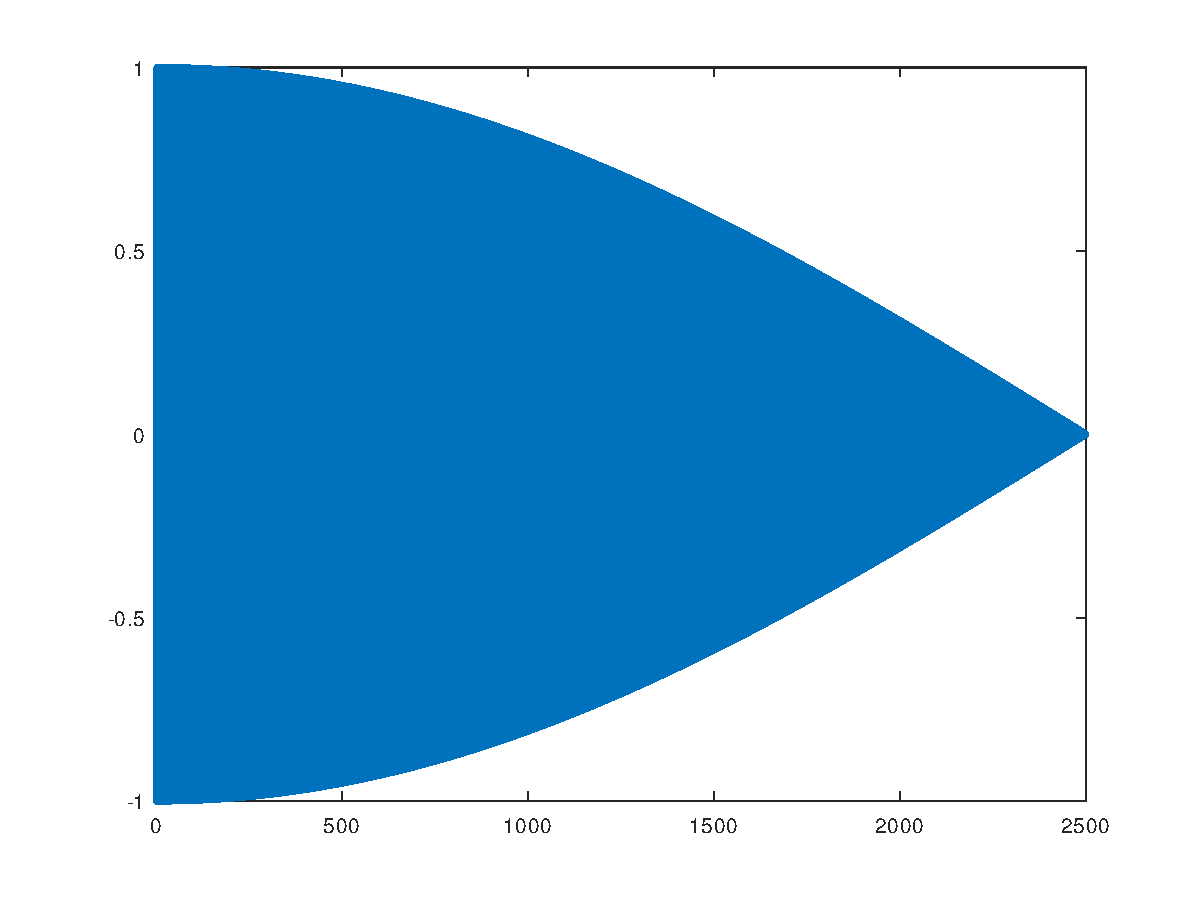
\includegraphics[
    width=\textwidth
    ]{papers/sgwt/images/dirac/dirac_fft_real.pdf}
    \vspace{-0pt}
    \caption{Fourier Transformation des Dirac-Stosses $\hat{\delta(x)}$ 
        aus~\cref{fig:sgwt:gft:dirac}.\label{fig:sgwt:gft:igft}}
    \end{minipage}
\end{figure}

\begin{figure}
    \centering
    \begin{minipage}[b]{0.49\textwidth}
    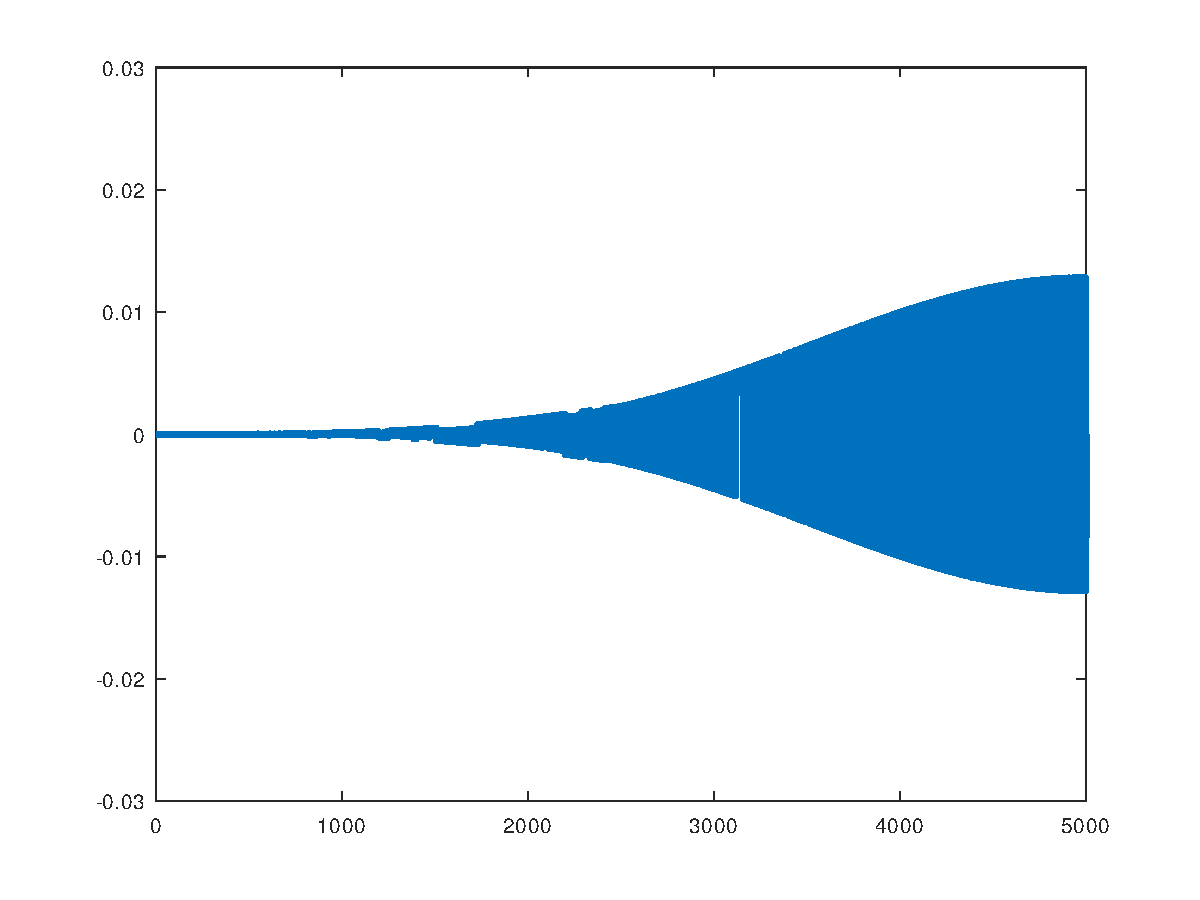
\includegraphics[
    width=\textwidth
    ]{papers/sgwt/images/dirac/dirac_gt1_gft.pdf}
    \vspace{-0pt}
    \caption{Darstellung eines Dirac-Stoss $\delta(x)$ mit maximal Wert $1$. 
        \label{fig:sgwt:gft:dirac}}
    \end{minipage}
    ~
    \begin{minipage}[b]{0.49\textwidth}
    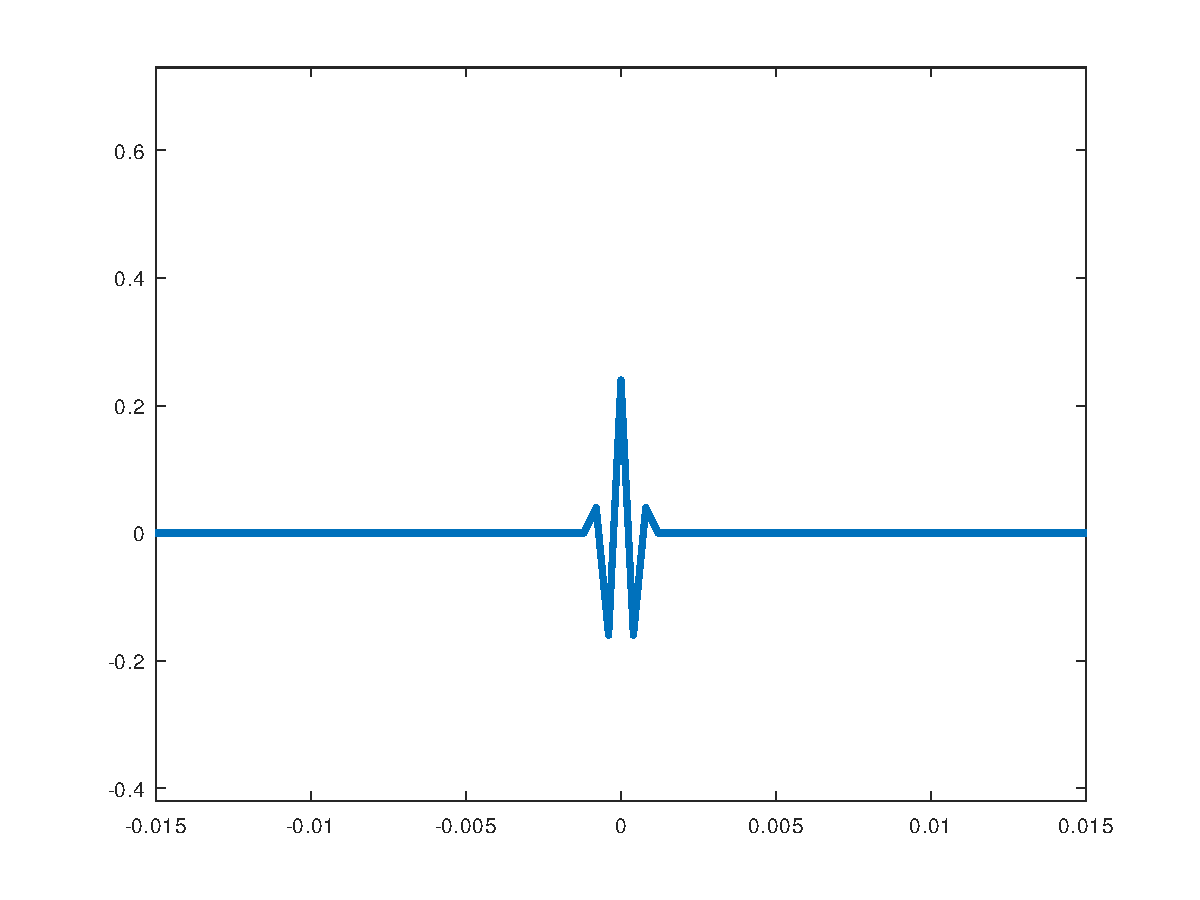
\includegraphics[
    width=\textwidth
    ]{papers/sgwt/images/dirac/dirac_gt1_igft.pdf}
    \vspace{-0pt}
    \caption{Fourier Transformation des Dirac-Stosses $\hat{\delta(x)}$ 
        aus~\cref{fig:sgwt:gft:dirac}.\label{fig:sgwt:gft:igft}}
    \end{minipage}
    ~
    \begin{minipage}[b]{0.49\textwidth}
    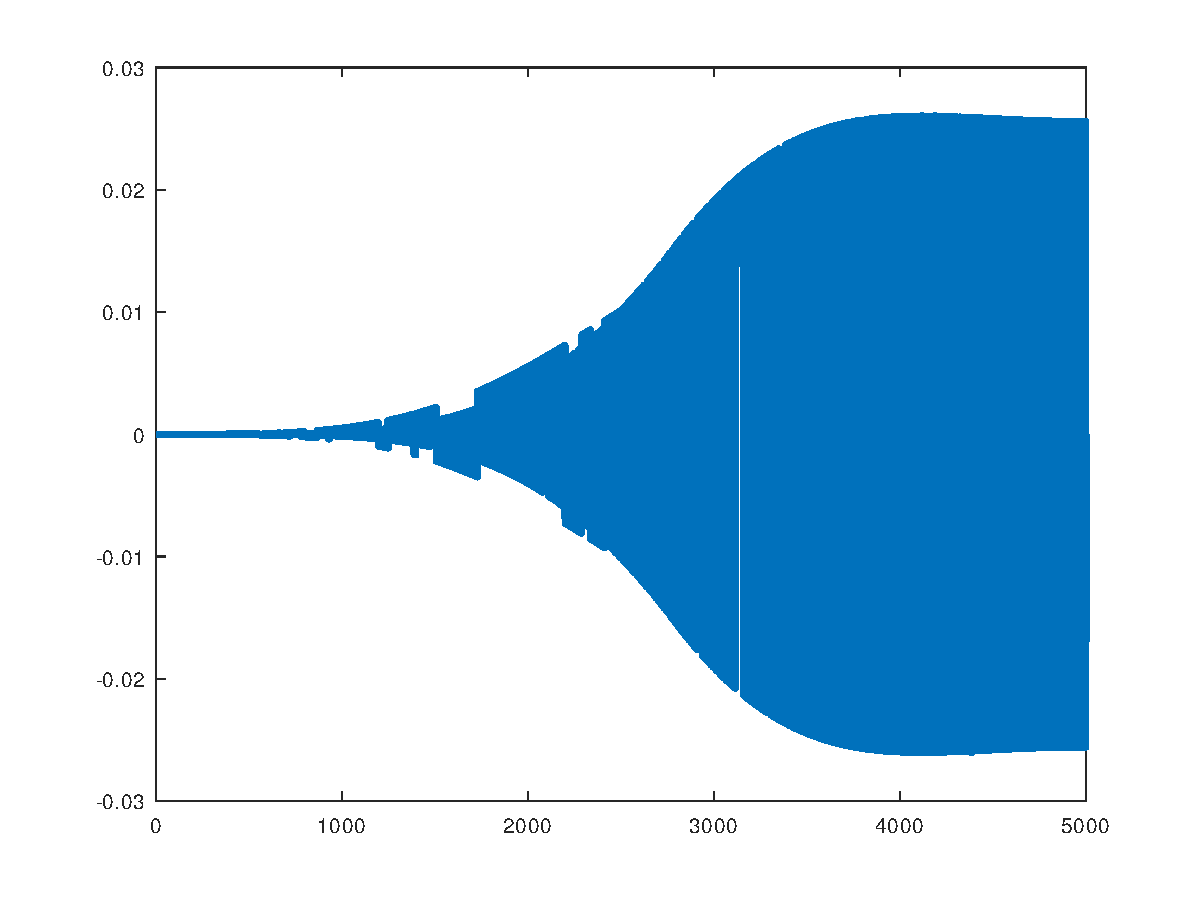
\includegraphics[
    width=\textwidth
    ]{papers/sgwt/images/dirac/dirac_gt2_gft.pdf}
    \vspace{-0pt}
    \caption{Fourier Transformation des Dirac-Stosses $\hat{\delta(x)}$ 
        aus~\cref{fig:sgwt:gft:dirac}.\label{fig:sgwt:gft:gft}}
    \end{minipage}
    ~
    \begin{minipage}[b]{0.49\textwidth}
    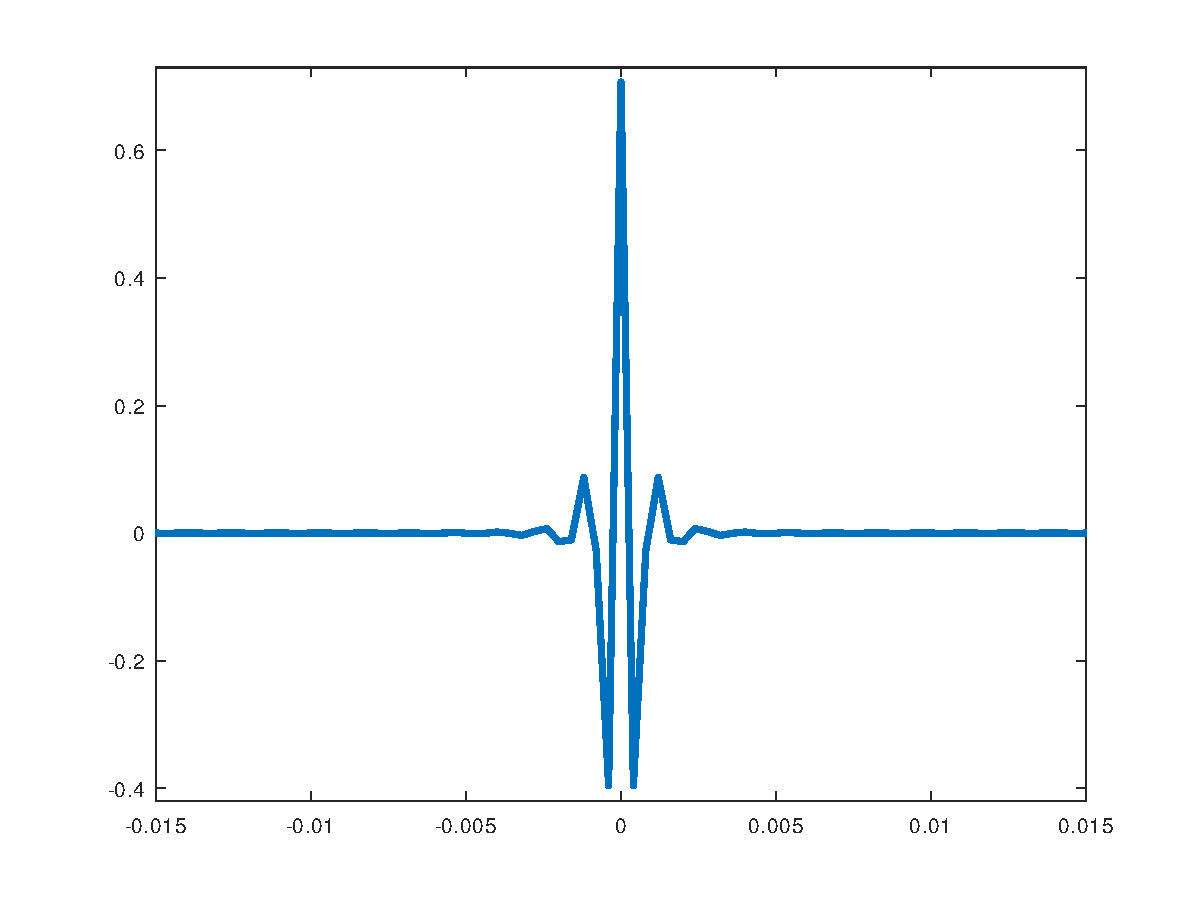
\includegraphics[
    width=\textwidth
    ]{papers/sgwt/images/dirac/dirac_gt2_igft.pdf}
    \vspace{-0pt}
    \caption{Fourier Transformation des Dirac-Stosses $\hat{\delta(x)}$ 
        aus~\cref{fig:sgwt:gft:dirac}.\label{fig:sgwt:gft:ggft}}
    \end{minipage}
    ~
    \begin{minipage}[b]{0.49\textwidth}
    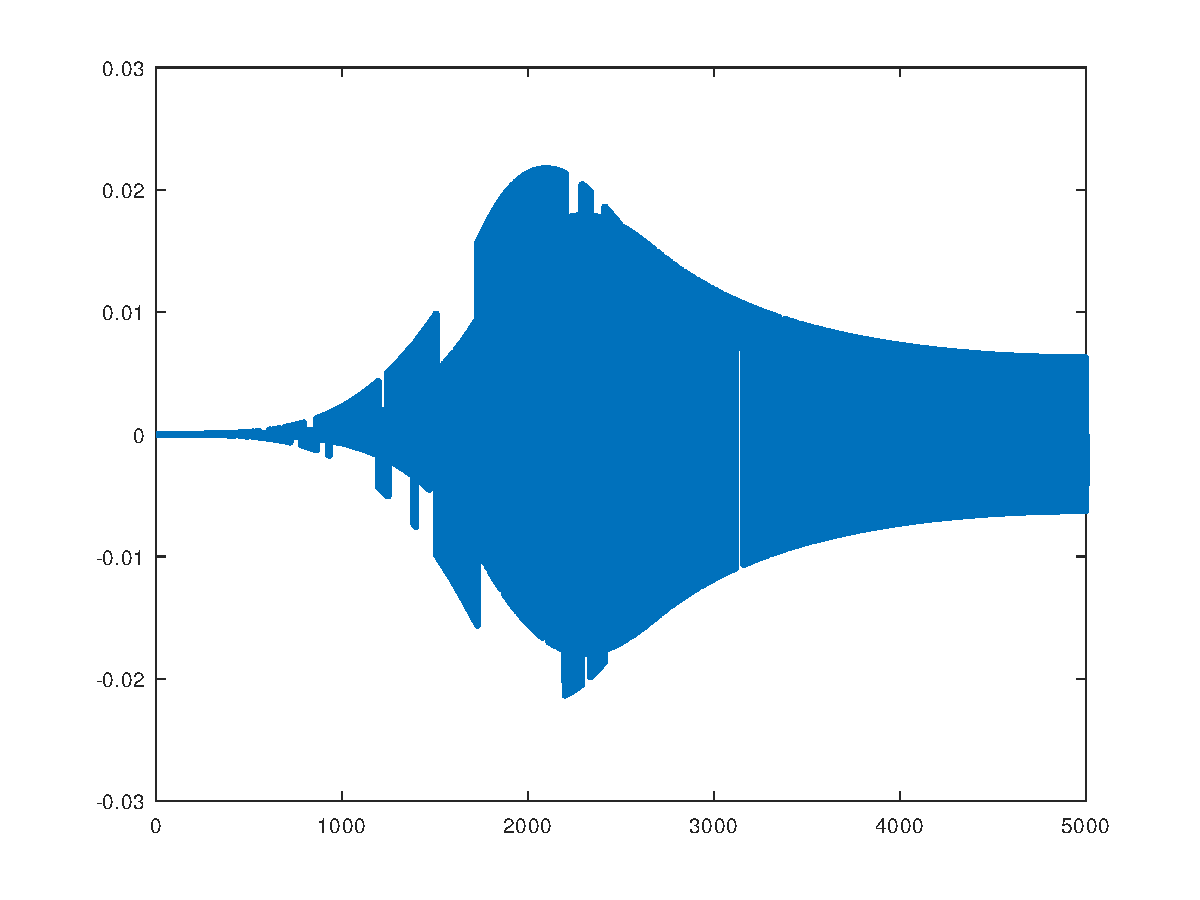
\includegraphics[
    width=\textwidth
    ]{papers/sgwt/images/dirac/dirac_gt3_gft.pdf}
    \vspace{-0pt}
    \caption{Fourier Transformation des Dirac-Stosses $\hat{\delta(x)}$ 
        aus~\cref{fig:sgwt:gft:dirac}.\label{fig:sgwt:gft:ggft}}
    \end{minipage}
    ~
    \begin{minipage}[b]{0.49\textwidth}
    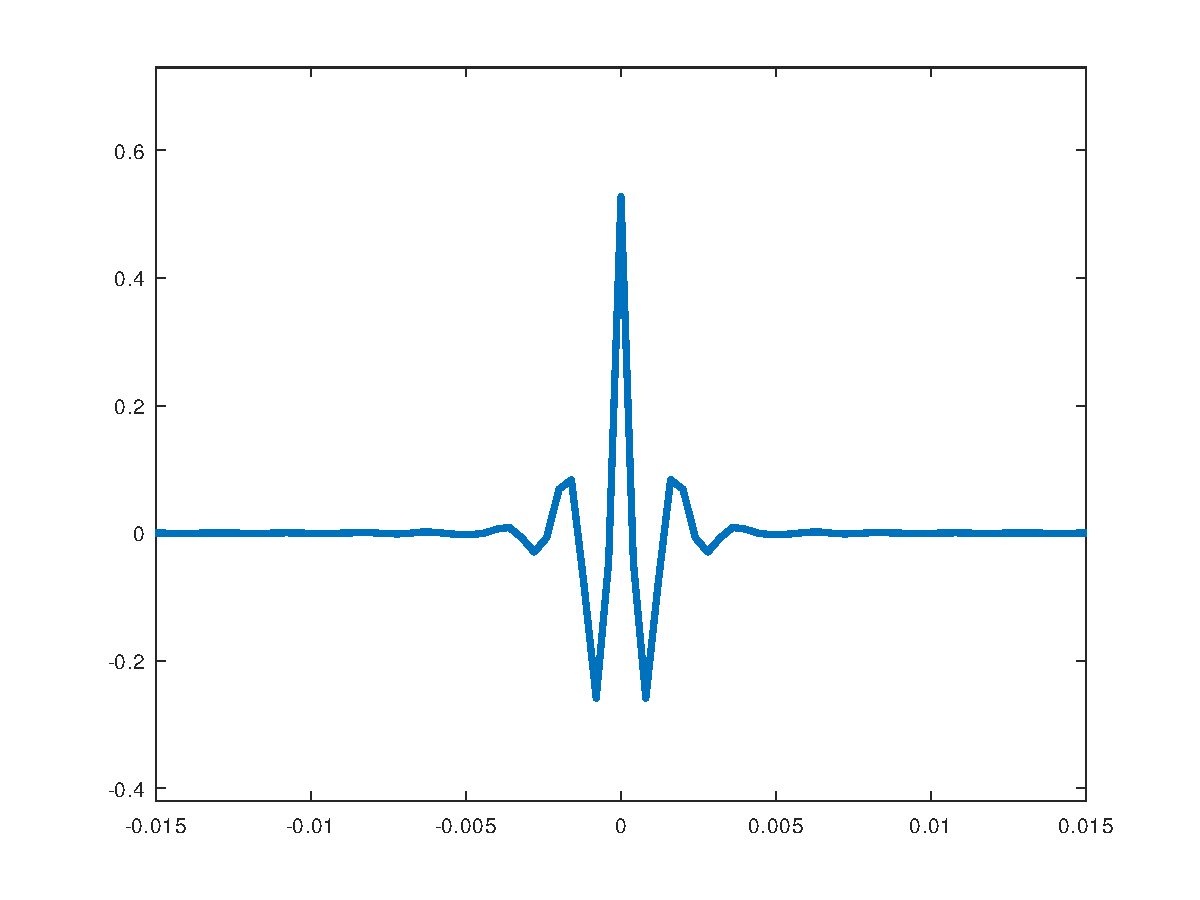
\includegraphics[
    width=\textwidth
    ]{papers/sgwt/images/dirac/dirac_gt3_igft.pdf}
    \vspace{-0pt}
    \caption{Fourier Transformation des Dirac-Stosses $\hat{\delta(x)}$ 
        aus~\cref{fig:sgwt:gft:dirac}.\label{fig:sgwt:gft:ggft}}
    \end{minipage}
\end{figure}



\begin{figure}
    \centering
    \begin{minipage}[b]{0.49\textwidth}
    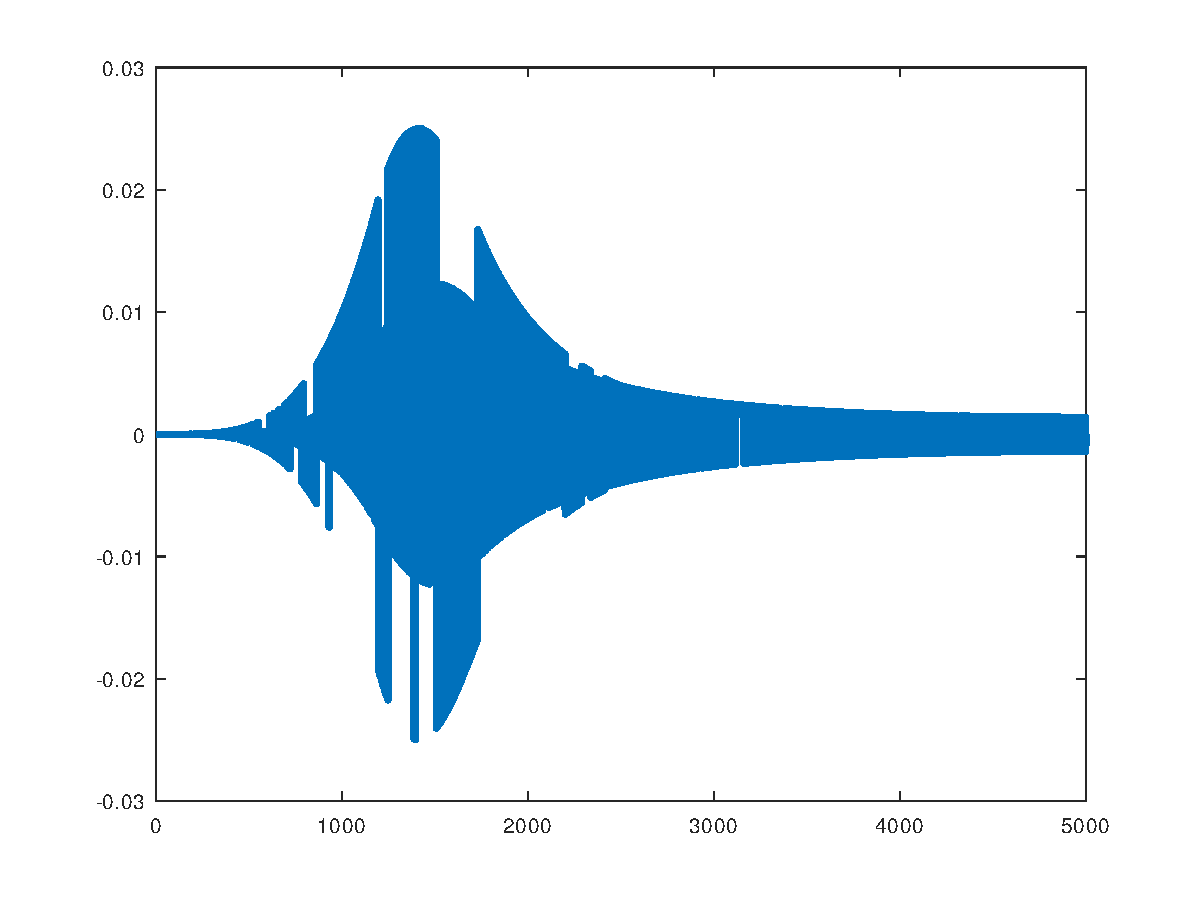
\includegraphics[
    width=\textwidth
    ]{papers/sgwt/images/dirac/dirac_gt4_gft.pdf}
    \vspace{-0pt}
    \caption{Darstellung eines Dirac-Stoss $\delta(x)$ mit maximal Wert $1$. 
        \label{fig:sgwt:gft:dirac}}
    \end{minipage}
    ~
    \begin{minipage}[b]{0.49\textwidth}
    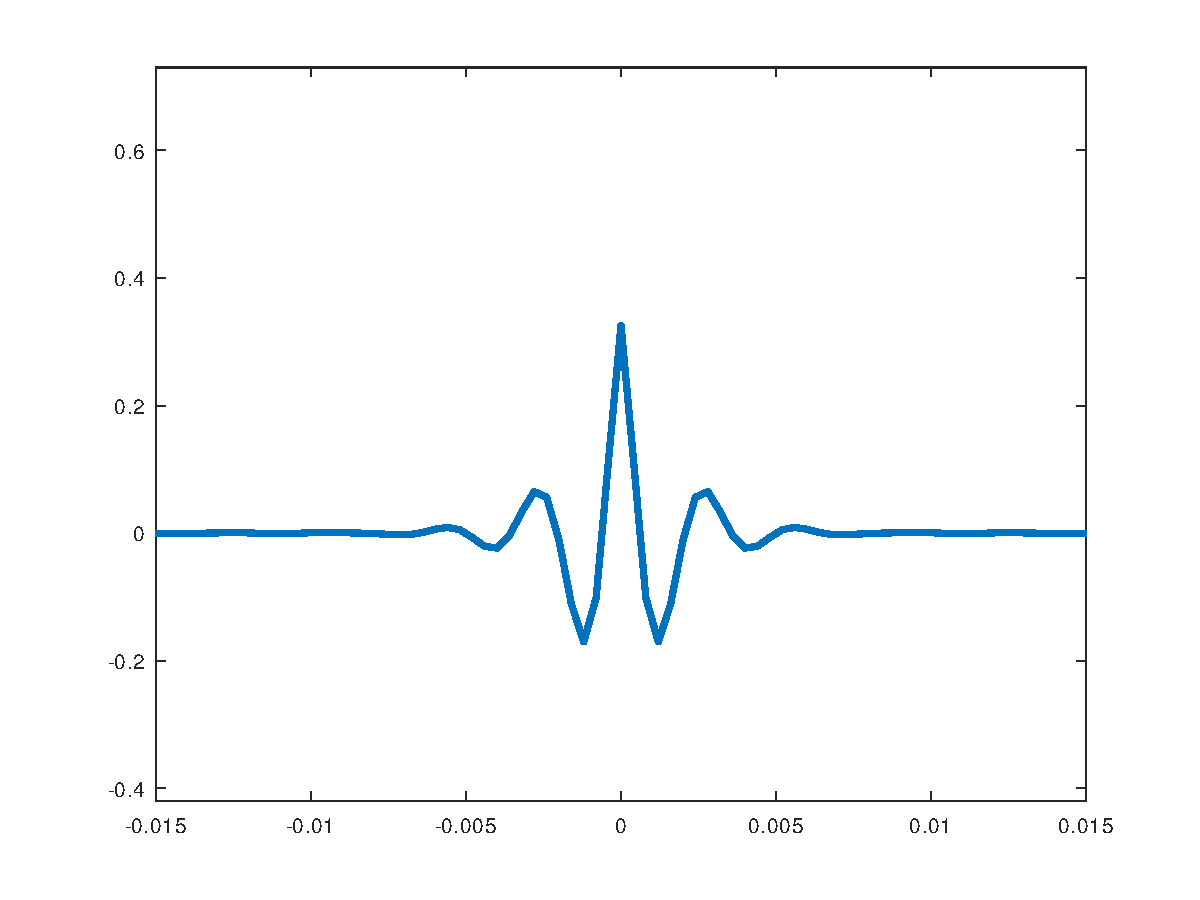
\includegraphics[
    width=\textwidth
    ]{papers/sgwt/images/dirac/dirac_gt4_igft.pdf}
    \vspace{-0pt}
    \caption{Fourier Transformation des Dirac-Stosses $\hat{\delta(x)}$ 
        aus~\cref{fig:sgwt:gft:dirac}.\label{fig:sgwt:gft:igft}}
    \end{minipage}
    ~
    \begin{minipage}[b]{0.49\textwidth}
    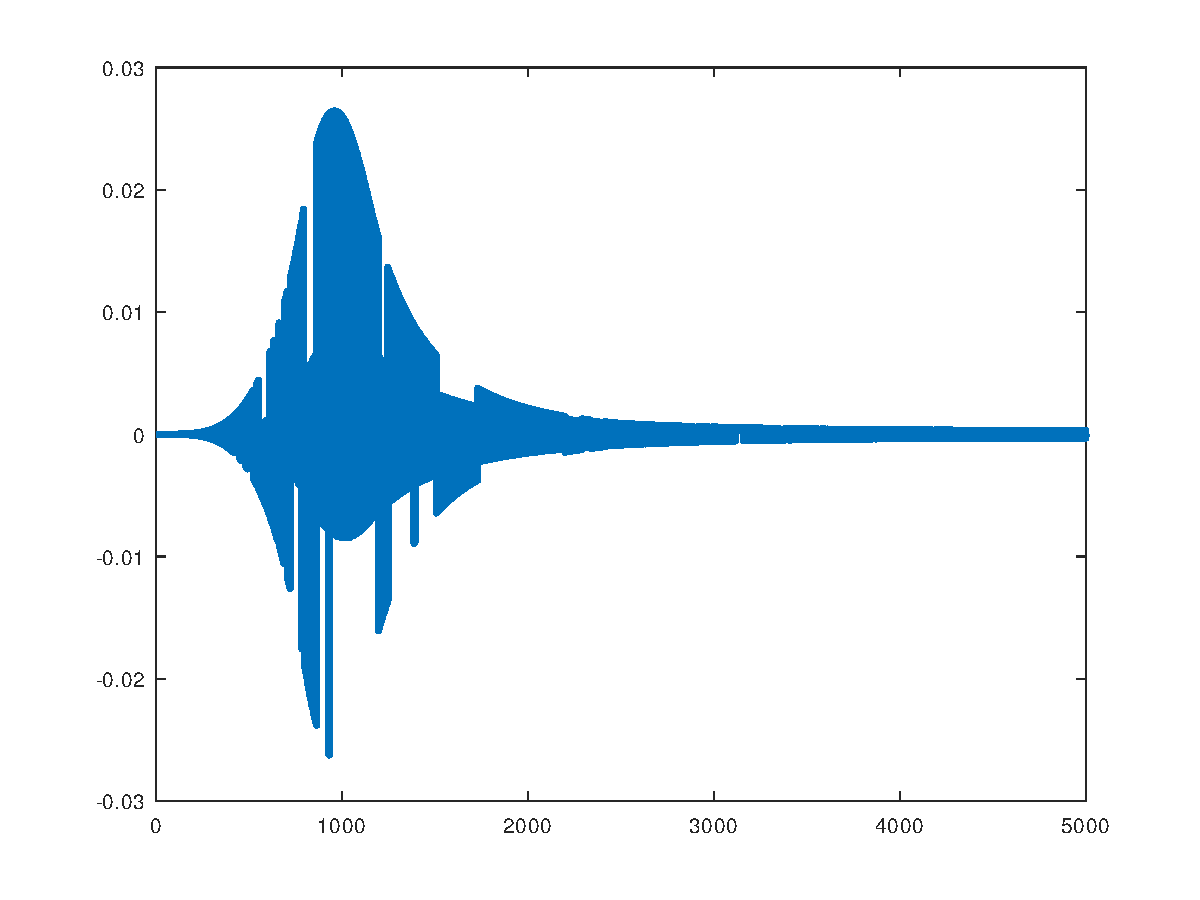
\includegraphics[
    width=\textwidth
    ]{papers/sgwt/images/dirac/dirac_gt5_gft.pdf}
    \vspace{-0pt}
    \caption{Fourier Transformation des Dirac-Stosses $\hat{\delta(x)}$ 
        aus~\cref{fig:sgwt:gft:dirac}.\label{fig:sgwt:gft:gft}}
    \end{minipage}
    ~
    \begin{minipage}[b]{0.49\textwidth}
    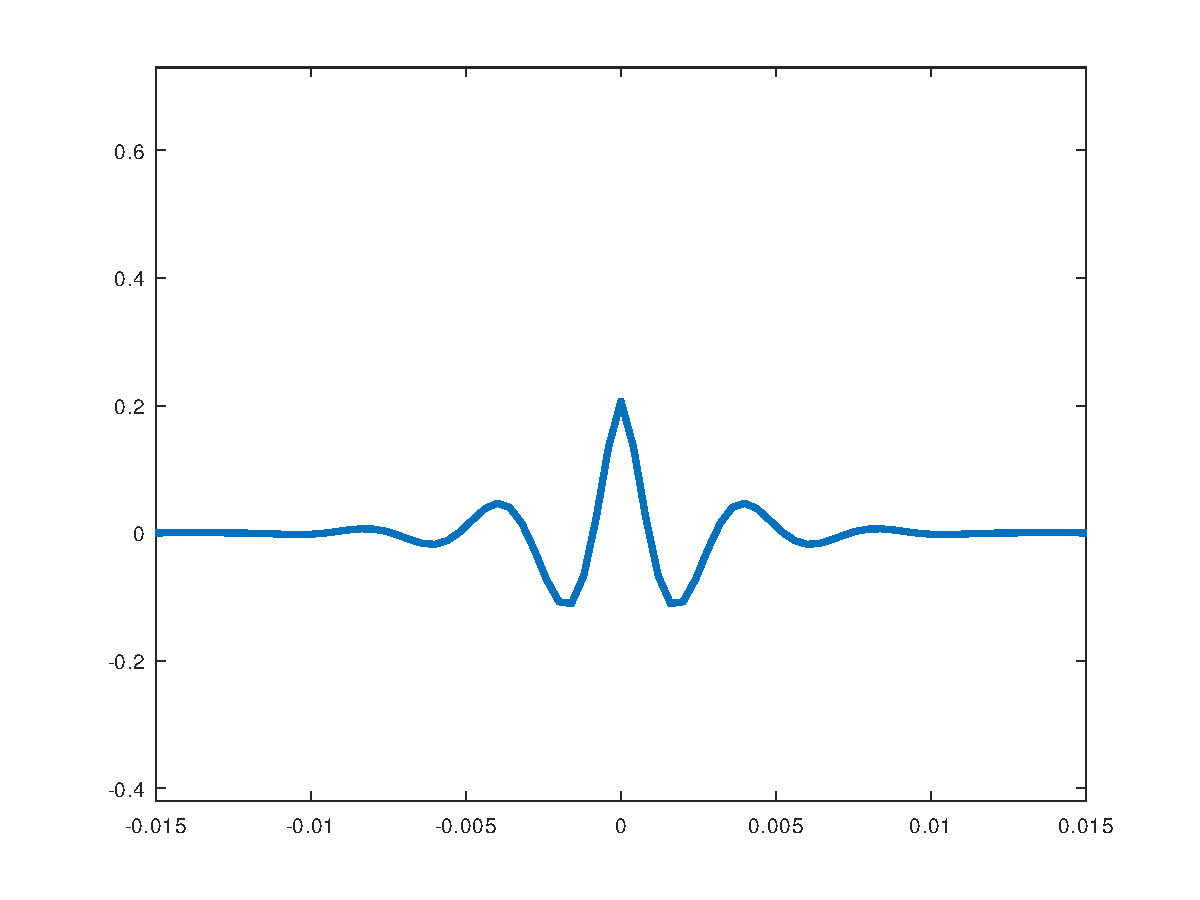
\includegraphics[
    width=\textwidth
    ]{papers/sgwt/images/dirac/dirac_gt5_igft.pdf}
    \vspace{-0pt}
    \caption{Fourier Transformation des Dirac-Stosses $\hat{\delta(x)}$ 
        aus~\cref{fig:sgwt:gft:dirac}.\label{fig:sgwt:gft:ggft}}
    \end{minipage}
    ~
    \begin{minipage}[b]{0.49\textwidth}
    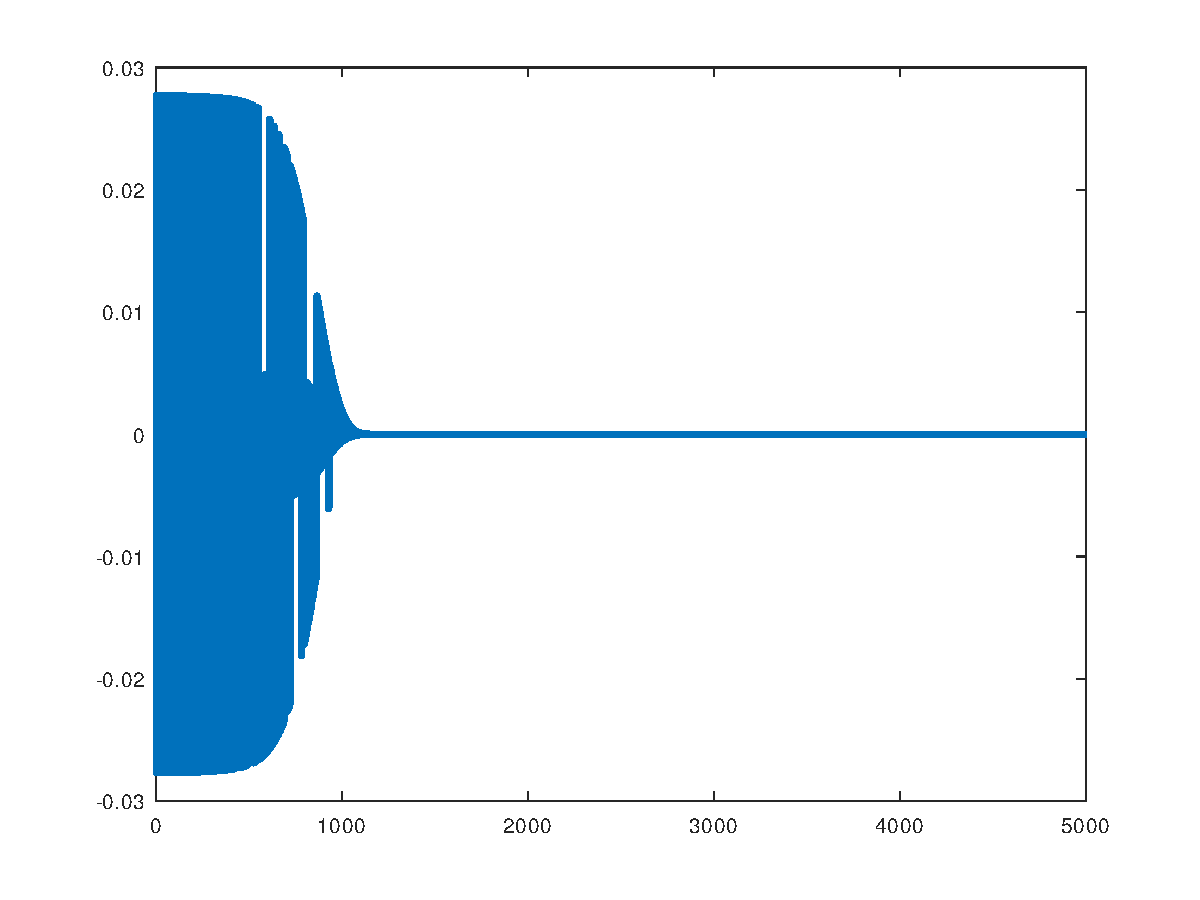
\includegraphics[
    width=\textwidth
    ]{papers/sgwt/images/dirac/dirac_h_gft.pdf}
    \vspace{-0pt}
    \caption{Fourier Transformation des Dirac-Stosses $\hat{\delta(x)}$ 
        aus~\cref{fig:sgwt:gft:dirac}.\label{fig:sgwt:gft:ggft}}
    \end{minipage}
    ~
    \begin{minipage}[b]{0.49\textwidth}
    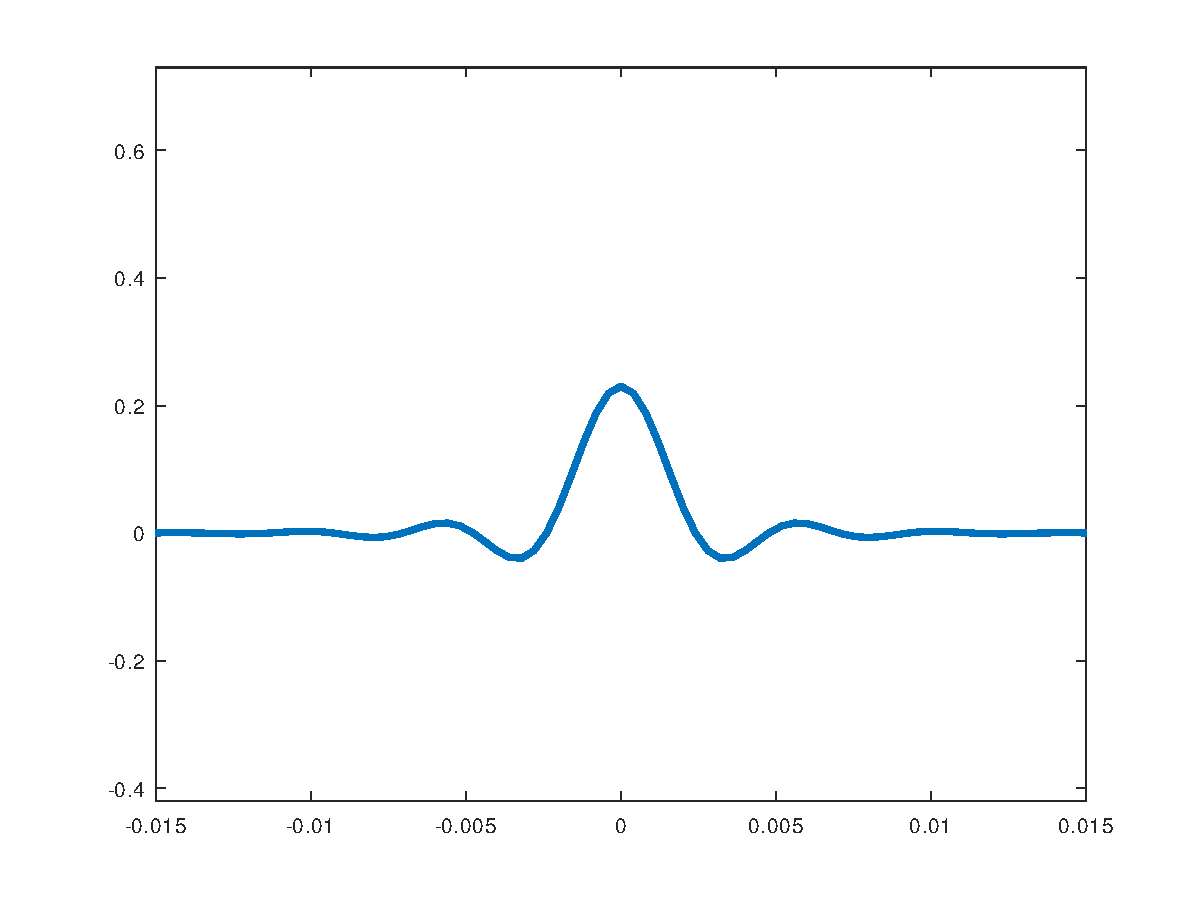
\includegraphics[
    width=\textwidth
    ]{papers/sgwt/images/dirac/dirac_h_igft.pdf}
    \vspace{-0pt}
    \caption{Fourier Transformation des Dirac-Stosses $\hat{\delta(x)}$ 
        aus~\cref{fig:sgwt:gft:dirac}.\label{fig:sgwt:gft:ggft}}
    \end{minipage}
\end{figure}

\begin{figure}
    \centering
    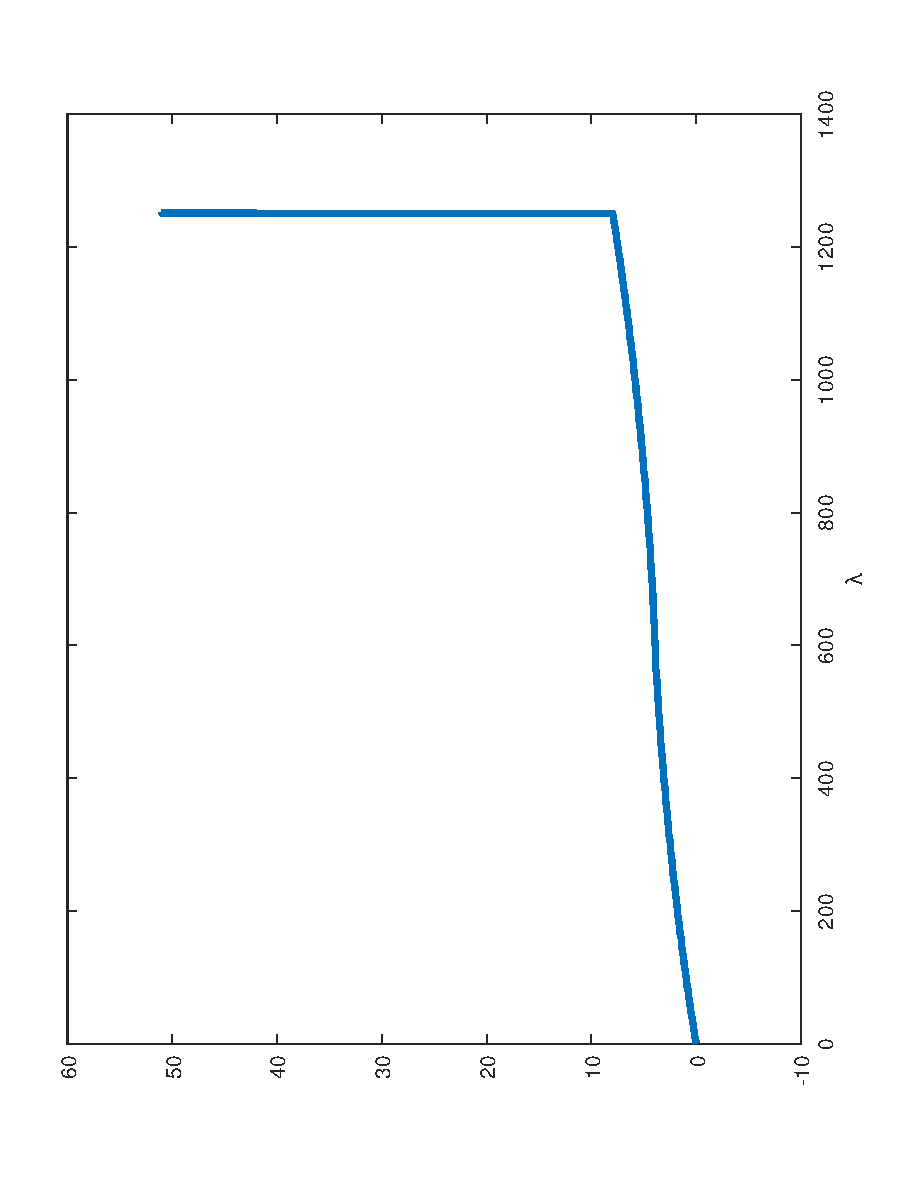
\includegraphics[
    angle=-90,
    origin=c,
    scale=0.6
    ]{papers/sgwt/images/wavelets/lambda.pdf}
    \vspace{-50pt}
    \caption{Eigenwerte $\lambda$ eines Kugelgraphen mit 1252 Knoten. 
    \label{fig:sgwt:wavelets:sphere:lambda}}
\end{figure}

\begin{figure}
    \begin{minipage}[b]{0.49\textwidth}
        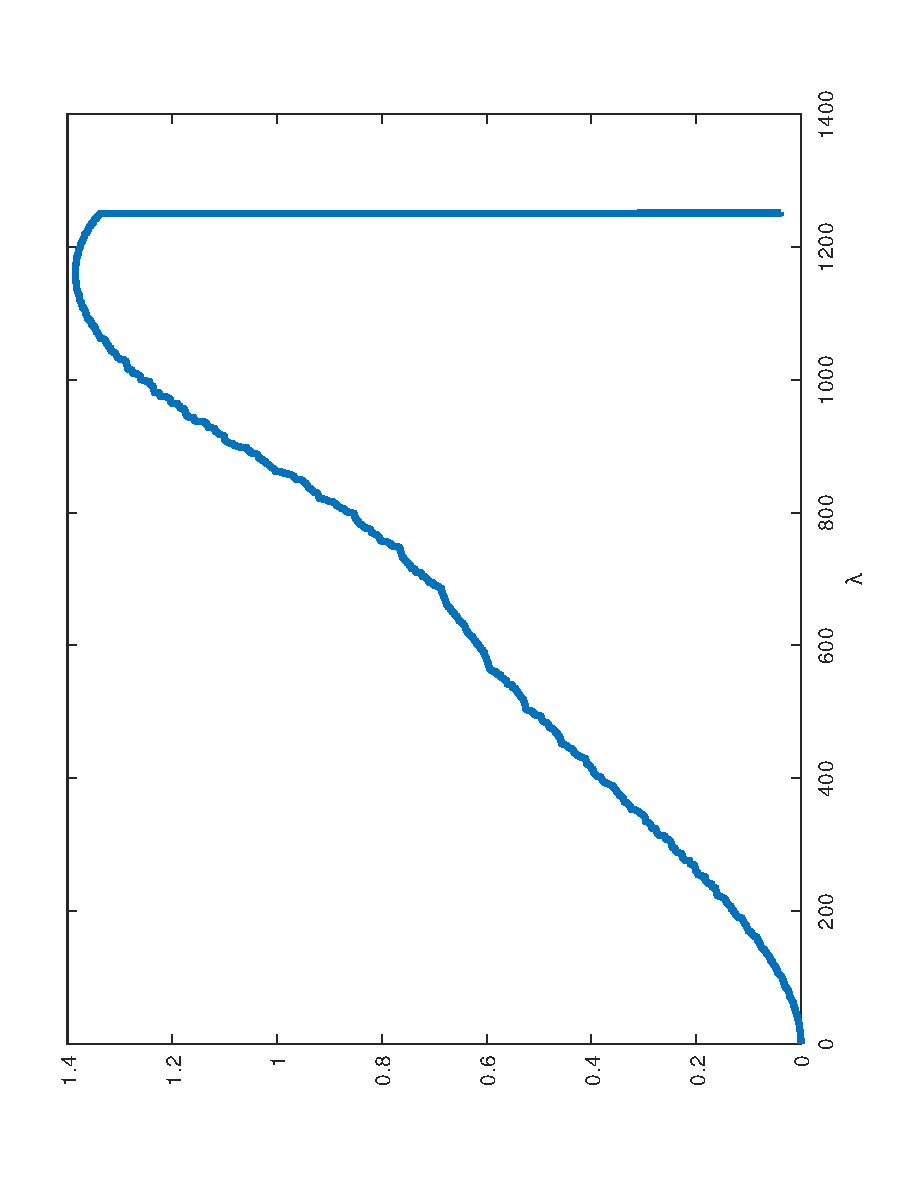
\includegraphics[
        angle=-90,
        origin=c,
        width=\textwidth]{papers/sgwt/images/wavelets/gt1.pdf}
        \vspace{-45pt}
        \caption{Die Kernelfunktion $g(t_1\lambda)$ eines Kugelgraphen mit 1252 
        Knoten und $t_1 = 0.2$.}
        \label{fig:sgwt:wavelets:sphere:gt1}
    \end{minipage}
    ~
    \begin{minipage}[b]{0.49\textwidth}
        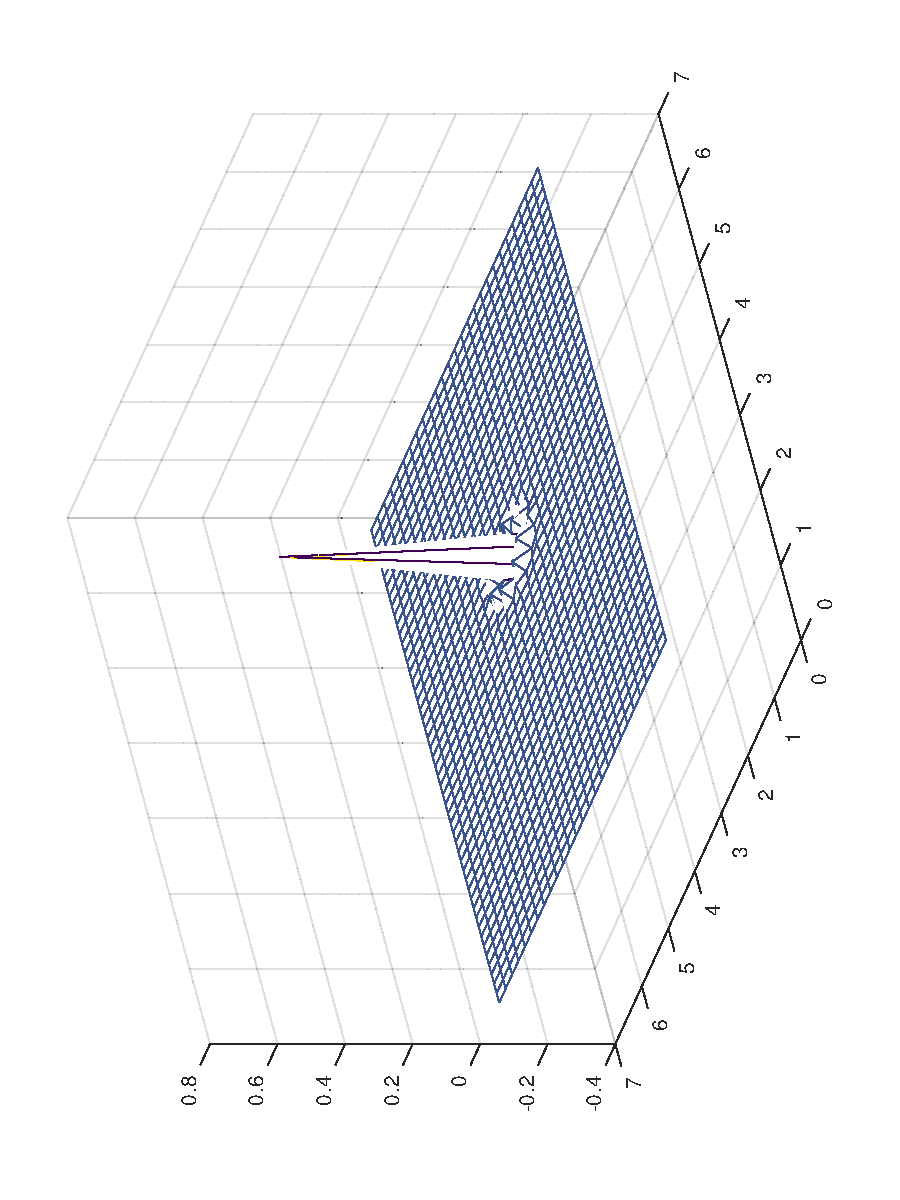
\includegraphics[
        angle=-90,
        origin=c,
        width=\textwidth]{papers/sgwt/images/wavelets/psi_t1_50_25_630_flat.pdf}
        \vspace{-45pt}
        \caption{$\psi_1(v_{630})$-Wavelet eines Kugelgraphen mit 1252 Knoten.}
        \label{fig:sgwt:wavelets:sphere:psi1:flat}
    \end{minipage}
    ~
    \begin{minipage}[b]{\textwidth}
        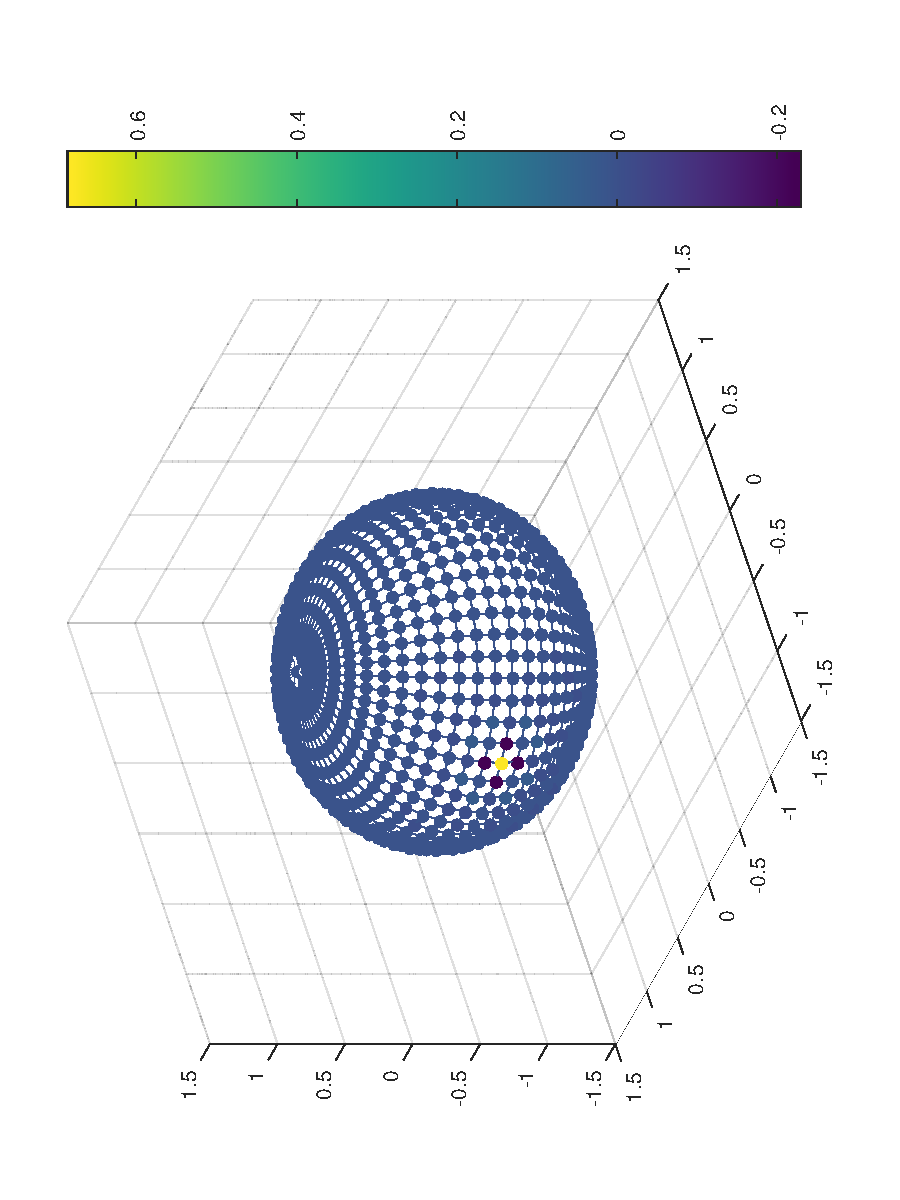
\includegraphics[
        angle=-90,
        origin=c,
        width=\textwidth]{papers/sgwt/images/wavelets/psi_t1_50_25_630.pdf}
        \vspace{-45pt}
        \caption{$\psi_1(v_{630})$-Wavelet eines Kugelgraphen mit 1252 Knoten 
        und $t = 0.42295$.}
        \label{fig:sgwt:wavelets:sphere:psi1}
    \end{minipage}
\end{figure}

\begin{figure}
    \begin{minipage}[b]{0.49\textwidth}
        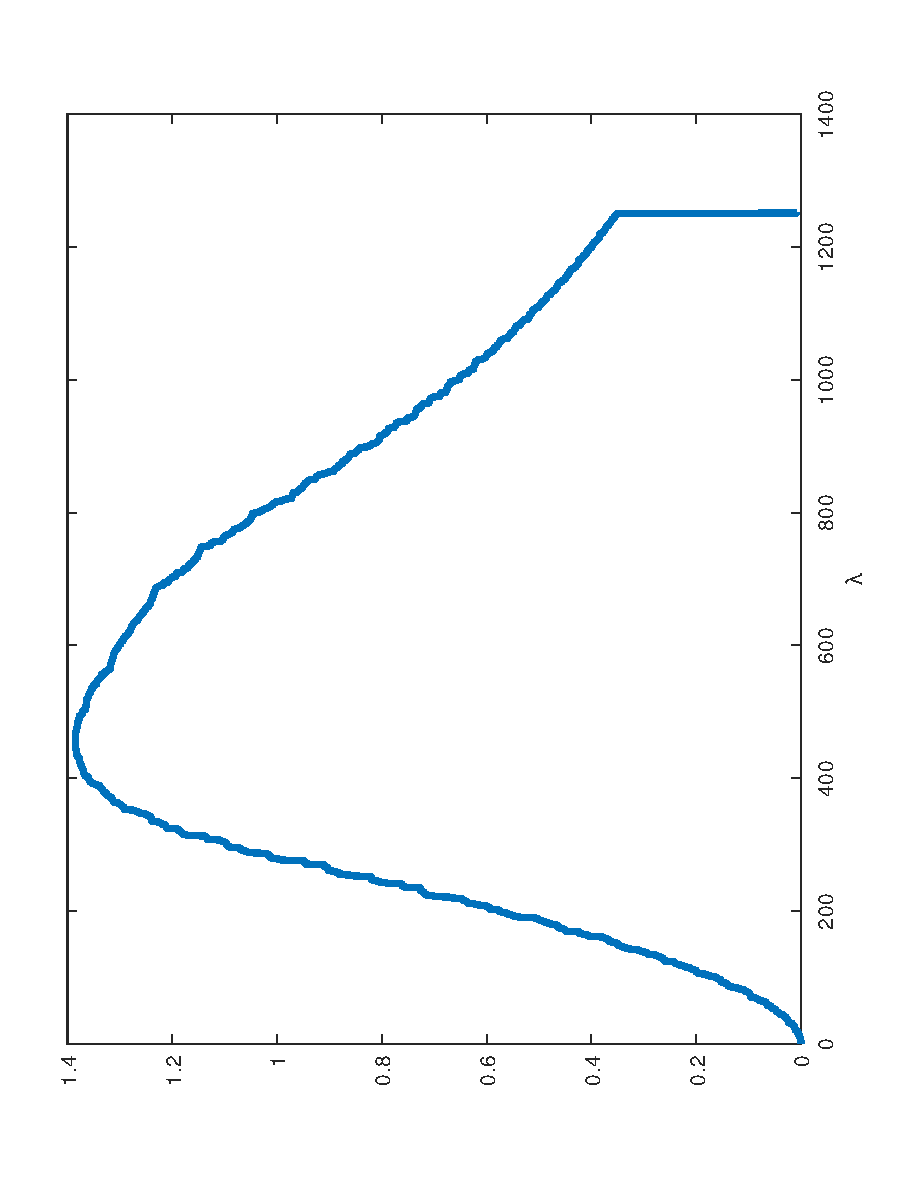
\includegraphics[
        angle=-90,
        origin=c,
        width=\textwidth]{papers/sgwt/images/wavelets/gt2.pdf}
        \vspace{-45pt}
        \caption{Die Kernelfunktion $g(t_2\lambda)$ eines Kugelgraphen mit 1252 
            Knoten und $t_2 = 0.42295$.}
        \label{fig:sgwt:wavelets:sphere:gt2}
    \end{minipage}
    ~
    \begin{minipage}[b]{0.49\textwidth}
        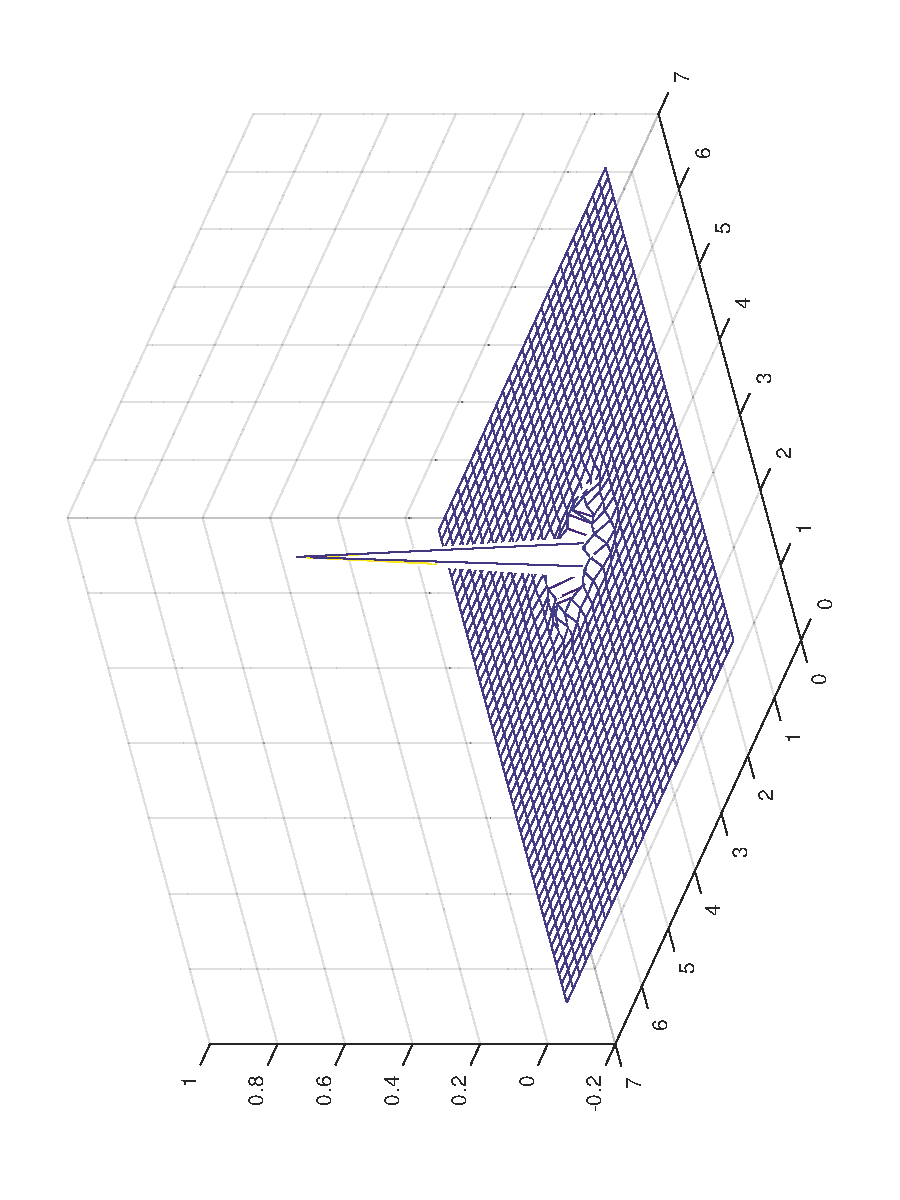
\includegraphics[
        angle=-90,
        origin=c,
        width=\textwidth]{papers/sgwt/images/wavelets/psi_t2_50_25_630_flat.pdf}
        \vspace{-45pt}
        \caption{$\psi_2(v_{630})$-Wavelet eines Kugelgraphen mit 1252 Knoten.}
        \label{fig:sgwt:wavelets:sphere:psi2:flat}
    \end{minipage}
    ~
    \begin{minipage}[b]{\textwidth}
        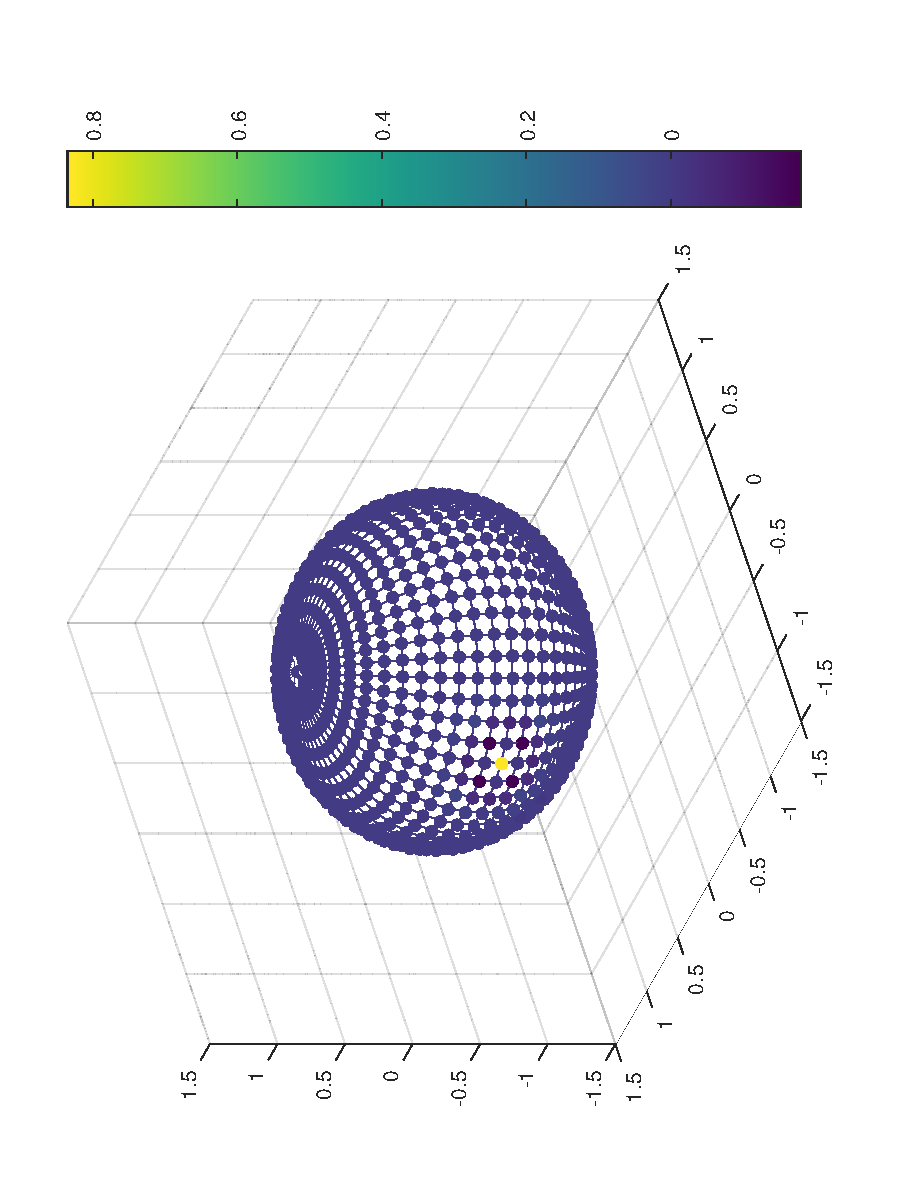
\includegraphics[
        angle=-90,
        origin=c,
        width=\textwidth]{papers/sgwt/images/wavelets/psi_t2_50_25_630.pdf}
        \vspace{-45pt}
        \caption{$\psi_2(v_{630})$-Wavelet eines Kugelgraphen mit 1252 Knoten.}
        \label{fig:sgwt:wavelets:sphere:psi2}
    \end{minipage}
\end{figure}

\begin{figure}
    \begin{minipage}[b]{0.49\textwidth}
        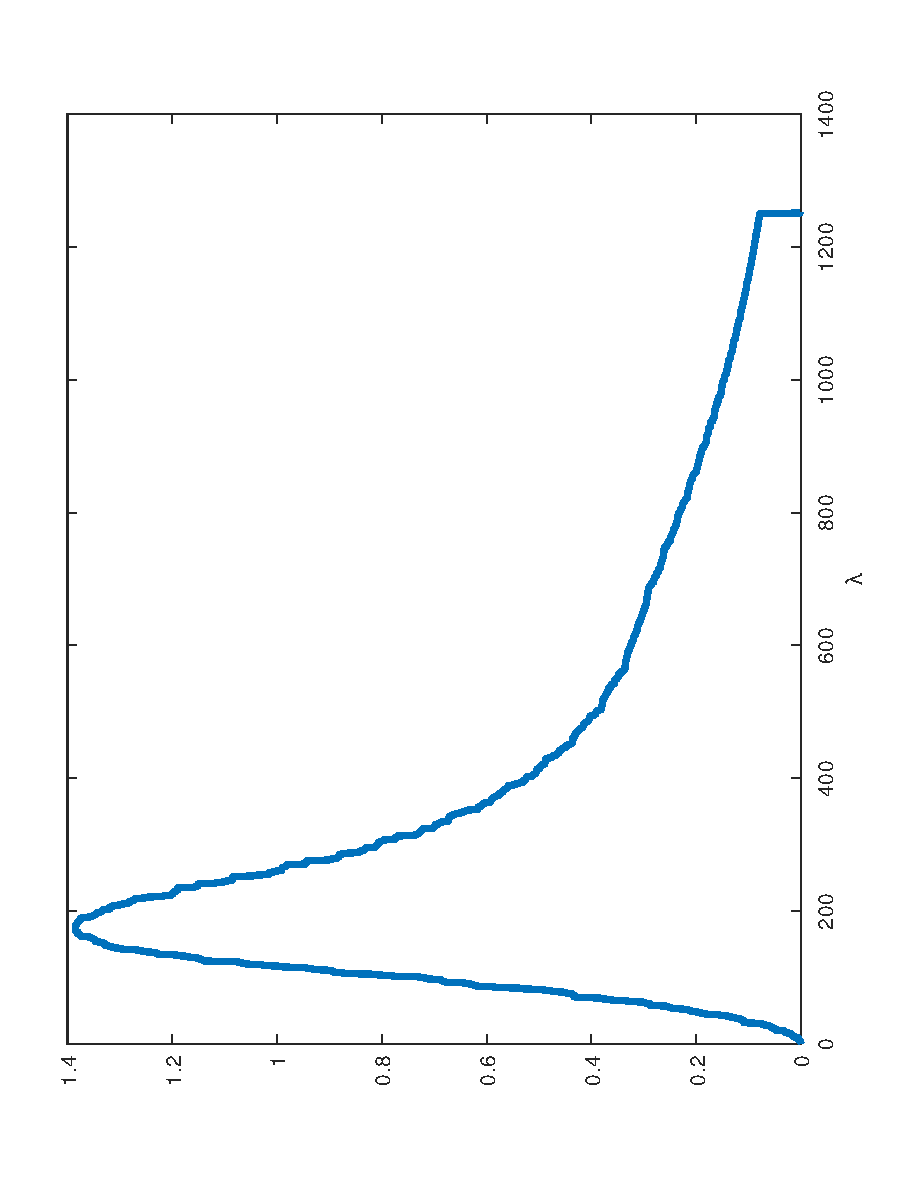
\includegraphics[
        angle=-90,
        origin=c,
        width=\textwidth]{papers/sgwt/images/wavelets/gt3.pdf}
        \vspace{-45pt}
        \caption{Die Kernelfunktion $g(t_3\lambda)$ eines Kugelgraphen mit 1252 
            Knoten und $t_3 = 0.89443$.}
        \label{fig:sgwt:wavelets:sphere:gt3}
    \end{minipage}
    ~
    \begin{minipage}[b]{0.49\textwidth}
        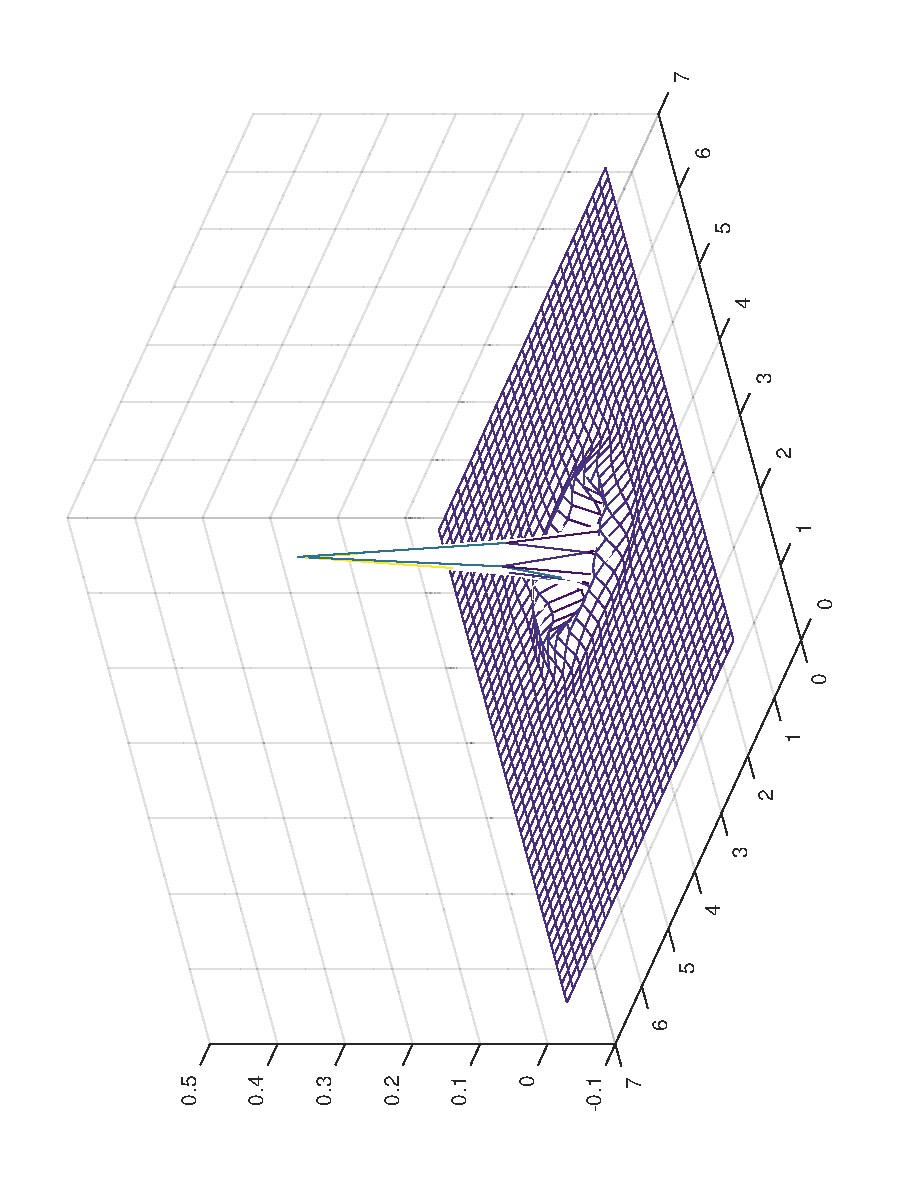
\includegraphics[
        angle=-90,
        origin=c,
        width=\textwidth]{papers/sgwt/images/wavelets/psi_t3_50_25_630_flat.pdf}
        \vspace{-45pt}
        \caption{$\psi_3(v_{630})$-Wavelet eines Kugelgraphen mit 1252 Knoten.}
        \label{fig:sgwt:wavelets:sphere:psi3:flat}
    \end{minipage}
    ~
    \begin{minipage}[b]{\textwidth}
        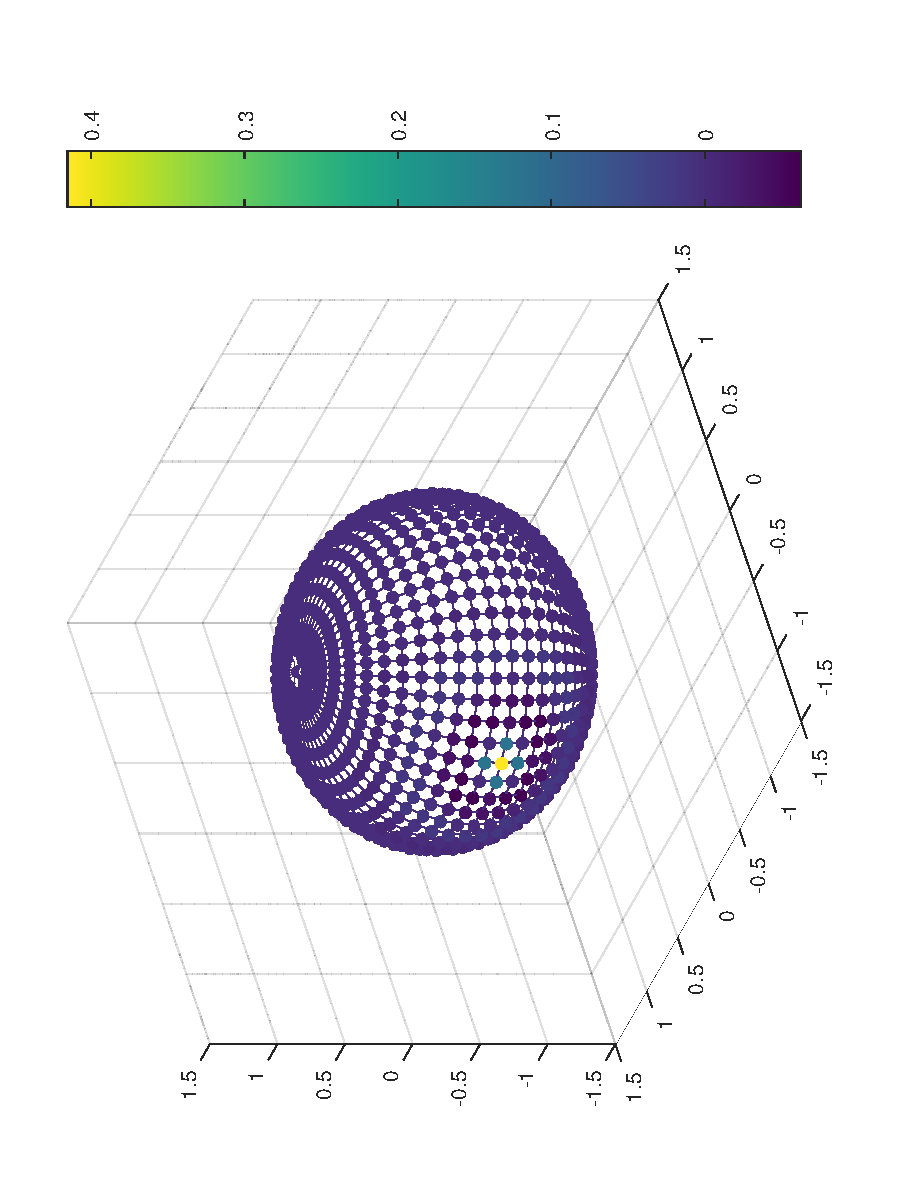
\includegraphics[
        angle=-90,
        origin=c,
        width=\textwidth]{papers/sgwt/images/wavelets/psi_t3_50_25_630.pdf}
        \vspace{-45pt}
        \caption{$\psi_3(v_{630})$-Wavelet eines Kugelgraphen mit 1252 Knoten.}
        \label{fig:sgwt:wavelets:sphere:psi3}
    \end{minipage}
\end{figure}

\begin{figure}
    \begin{minipage}[b]{0.49\textwidth}
        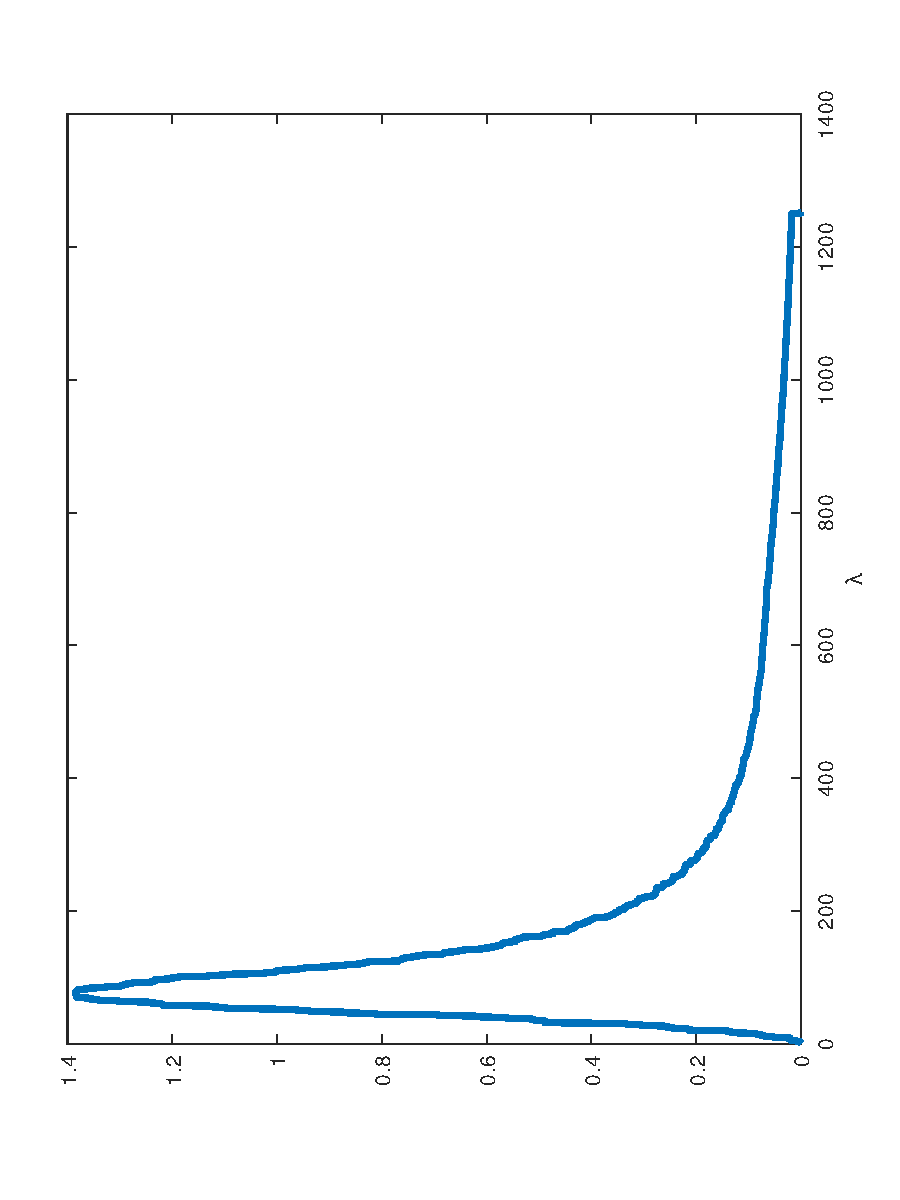
\includegraphics[
        angle=-90,
        origin=c,
        width=\textwidth]{papers/sgwt/images/wavelets/gt4.pdf}
        \vspace{-45pt}
        \caption{Die Kernelfunktion $g(t_4\lambda)$ eines Kugelgraphen mit 1252 
            Knoten und $t_4 = 1.89148$.}
        \label{fig:sgwt:wavelets:sphere:gt4}
    \end{minipage}
    ~
    \begin{minipage}[b]{0.49\textwidth}
        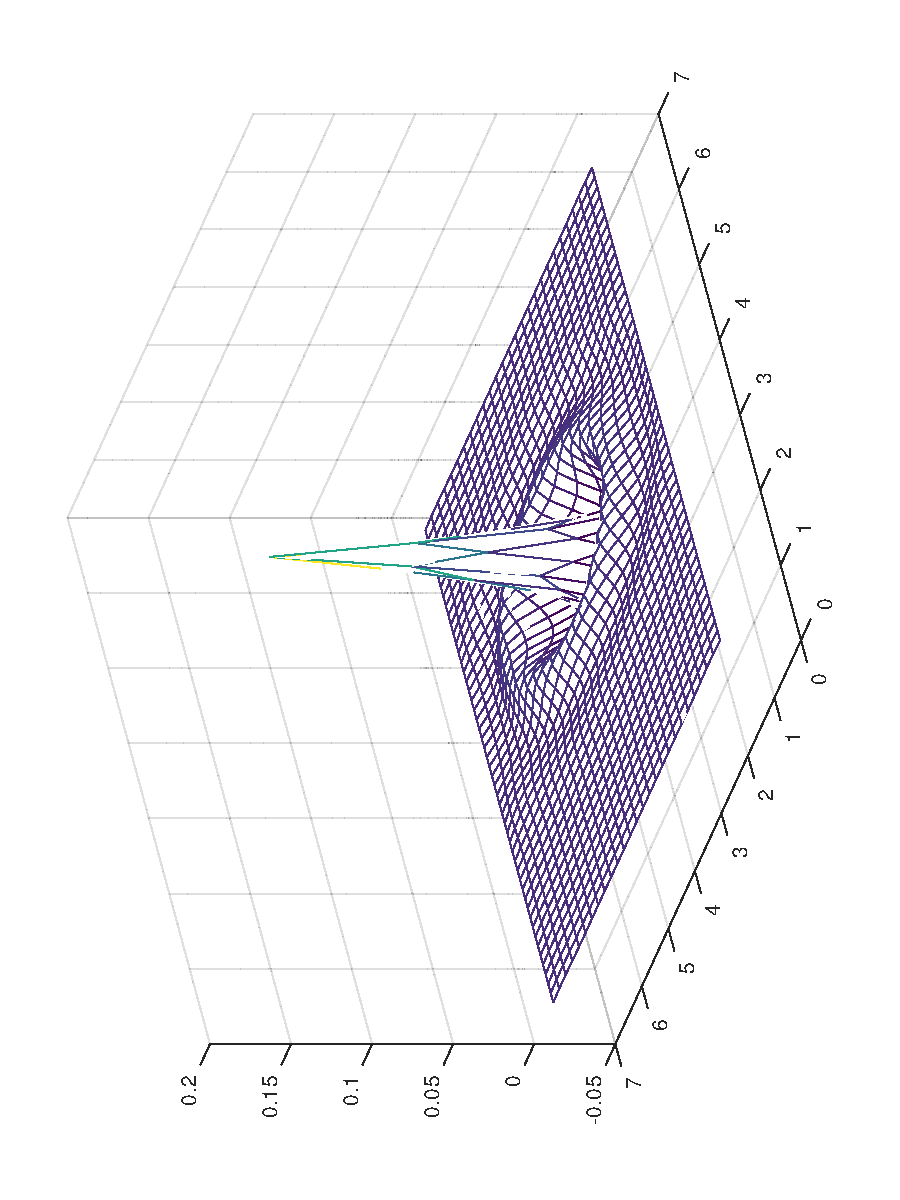
\includegraphics[
        angle=-90,
        origin=c,
        width=\textwidth]{papers/sgwt/images/wavelets/psi_t4_50_25_630_flat.pdf}
        \vspace{-45pt}
        \caption{$\psi_4(v_{630})$-Wavelet eines Kugelgraphen mit 1252 Knoten.}
        \label{fig:sgwt:wavelets:sphere:psi4:flat}
    \end{minipage}
    ~
    \begin{minipage}[b]{\textwidth}
        \includegraphics[
        angle=-90,
        origin=c,
        width=\textwidth]{papers/sgwt/images/wavelets/psi_t4_50_25_630.pdf}
        \vspace{-45pt}
        \caption{$\psi_4(v_{630})$-Wavelet eines Kugelgraphen mit 1252 Knoten.}
        \label{fig:sgwt:wavelets:sphere:psi4}
    \end{minipage}
\end{figure}

\begin{figure}
    \begin{minipage}[b]{0.49\textwidth}
        \includegraphics[
        angle=-90,
        origin=c,
        width=\textwidth]{papers/sgwt/images/wavelets/gt5.pdf}
        \vspace{-45pt}
        \caption{Die Kernelfunktion $g(t_5\lambda)$ eines Kugelgraphen mit 1252 
            Knoten und $t_5 = 4$.}
        \label{fig:sgwt:wavelets:sphere:gt5}
    \end{minipage}
    ~
    \begin{minipage}[b]{0.49\textwidth}
        \includegraphics[
        angle=-90,
        origin=c,
        width=\textwidth]{papers/sgwt/images/wavelets/psi_t5_50_25_630_flat.pdf}
        \vspace{-45pt}
        \caption{$\psi_5(v_{630})$-Wavelet eines Kugelgraphen mit 1252 Knoten.}
        \label{fig:sgwt:wavelets:sphere:psi5:flat}
    \end{minipage}
    ~
    \begin{minipage}[b]{\textwidth}
        \includegraphics[
        angle=-90,
        origin=c,
        width=\textwidth]{papers/sgwt/images/wavelets/psi_t5_50_25_630.pdf}
        \vspace{-45pt}
        \caption{$\psi_5(v_{630})$-Wavelet eines Kugelgraphen mit 1252 Knoten.}
        \label{fig:sgwt:wavelets:sphere:psi5}
    \end{minipage}
\end{figure}

\begin{figure}
    \begin{minipage}[b]{0.49\textwidth}
        \includegraphics[
        angle=-90,
        origin=c,
        width=\textwidth]{papers/sgwt/images/wavelets/h.pdf}
        \vspace{-45pt}
        \caption{Die Kernelfunktion $h(\lambda)$ eines Kugelgraphen mit 1252 
            Knoten.}
        \label{fig:sgwt:wavelets:sphere:h}
    \end{minipage}
    ~
    \begin{minipage}[b]{0.49\textwidth}
        \includegraphics[
        angle=-90,
        origin=c,
        width=\textwidth]{papers/sgwt/images/wavelets/phi_50_25_630_flat.pdf}
        \vspace{-45pt}
        \caption{$\phi(v_{630})$-Wavelet eines Kugelgraphen mit 1252 Knoten.}
        \label{fig:sgwt:wavelets:sphere:phi:flat}
    \end{minipage}
    ~
    \begin{minipage}[b]{\textwidth}
        \includegraphics[
        angle=-90,
        origin=c,
        width=\textwidth]{papers/sgwt/images/wavelets/phi_50_25_630.pdf}
        \vspace{-45pt}
        \caption{$\phi(v_{630})$-Wavelet eines Kugelgraphen mit 1252 Knoten.}
        \label{fig:sgwt:wavelets:sphere:phi}
    \end{minipage}
\end{figure}

\subsubsection{Kernelfunktionen}

Um dieses Problem zu l\"osen nehmen wir eine Kernelfunktion $g(\lambda)$, 
welche die Eigenschaften $g(0) = 0$ und $\lim_{\lambda\to\infty} g(x) = 0$ 
erf\"ullt. Mit Hilfe dieses Bandpasses k\"onnen wir die Eigenwerte bewusst 
delokalisieren. Wenn wir nun zus\"atzlich die Eigenwerte mit einem 
Skalierungsfaktor $t$ multiplizieren, erhalten wir auch eine 
M\"oglichkeit, das Spektrum zu verschieben. Obwohl $t$ ein kontinuierlicher 
Faktor ist, werden wir uns in der Praxis auf $J$ Faktoren, also eine endliche 
Anzahl $\{t_j\}^J_{j=1}$, beschr\"anken m\"ussen.

Wir haben jetzt nur noch das Problem, dass $\lambda_0 = 0$ gilt. Wir verlieren 
also den konstanten Anteil der zu analysierenden und synthetisierenden 
Funktion. Um das zu umgehen nehmen brauchen wir eine zus\"atzliche 
Kernelfunktion $h(\lambda)$ mit den Eigenschaften $h(0) > 0$ und 
$\lim_{\lambda\to\infty} = 0$.

Die in~\cref{sec:sgwt:spectralanalysis} vorgestellten Eigenfunktionen 
k\"onnen wir direkt nutzen um eine Graph Fourier Transformation zu definieren. 
Wir ersetzen bei der Fourier Transformation einfach die Exponentialfunktion 
oder Kugelfunktionen durch die Eigenvektoren der Laplace Matrix
\begin{equation*}
\hat{f} = \langle \chi, f \rangle = \sum_{n = 1}^{N} \chi^*(n)f(n).
\end{equation*}
Wenn wir, wie zum Beispiel in \texttt{octave} \"ublich, die Eigenvektoren als 
Spalten einer Matrix
\begin{equation}
\chi = 
\left[
\begin{pmatrix}\\\chi_0\\\\\end{pmatrix}
\begin{pmatrix}\\\chi_1\\\\\end{pmatrix}
\begin{pmatrix}\\\chi_2\\\\\end{pmatrix}
\cdots
\begin{pmatrix}\\\chi_{N-1}\\\\\end{pmatrix}
\right]
\end{equation}
zur Verf\"ugung haben, k\"onnen wir die Transformation 
einfach durch eine Matrix-Vektor Multiplikation ersetzen
\begin{equation*}
\hat{f} = \chi^* f.
\end{equation*}
Die R\"ucktransformation ist dann auch wieder analog der Fouriertheorie
\begin{equation*}
f = \chi \hat{f}.
\end{equation*}

\subsection{Graph Wavelets: Lokalisierung\label{subsec:sgwt:gwt:localizing}}

Mit der Graph Fourier Transformation k\"onnen wir nun Funktionen auf Graphen 
analysieren und dann auch wieder synthetisieren. Mit Hilfe von Wavelets haben 
wir aber bereits gesehen, dass damit auch eine Lokalisierung m\"oglich ist. 
Graphen haben da den Nachteil, dass die Knoten keine inh\"arente Reihenfolge 
haben. Es ist also nicht klar was mit $f(x - h)$ gemeint ist. Wir haben 
allerdings in~\cref{eq:sgwt:lambda:series} eine Reihenfolge f\"ur die 
Eigenwerte der Laplace Matrix eines Graphen definiert. Die Eigenwerte sind 
allerdings komplett lokalisiert, sie kommen also einem Dirac-Stoss an 
einem Knoten gleich.

\subsection{Graph Wavelets: Skalierung\label{subsec:sgwt:gwt:scaling}}

\subsection{Frames}

Mit $h(\lambda)$ und den $J$ skalierten $g(t\lambda)$ haben wir also $J + 1$ 
Kernelfunktionen f\"ur die Analyse und Synthese zur Verf\"ugung. Wir arbeiten 
also mit einem Frame. Die Grenzen sind dabei gegeben als
\begin{align*}
A &= \min_{\lambda \in \left[0, \lambda_{N-1}\right]} f(\lambda) \\
B &= \max_{\lambda \in \left[0, \lambda_{N-1}\right]} f(\lambda) \\
\text{mit } f(\lambda) &= h(\lambda)^2 + \sum_{j = 1}^{J} g(t_j\lambda)^2.
\end{align*}

\subsection{\texorpdfstring{$\psi_j$}{psi} und \texorpdfstring{$\phi$}{phi}}
Damit lassen sich nun unsere Wavelets $\psi_j$ und $\phi$ wie folgt konstruieren
\begin{align}
\psi_j = \chi \diag{g(t_j\lambda)} \chi' 
\label{eq:sgwt:psi}
\\
\phi = \chi \diag{h(\lambda)} \chi'.
\label{eq:sgwt:phi}
\end{align}
Zur Veranschaulichung sehen wir hier die Wavelets eines Kreisgraphen 
in~\cref{fig:sgwt:wavelets:ring0,fig:sgwt:wavelets:ring1,fig:sgwt:wavelets:ring2,fig:sgwt:wavelets:ring3,fig:sgwt:wavelets:ring4,fig:sgwt:wavelets:ring5},
 eines Streckengraphen 
in~\cref{fig:sgwt:wavelets:line0,fig:sgwt:wavelets:line1,fig:sgwt:wavelets:line2,fig:sgwt:wavelets:line3,fig:sgwt:wavelets:line4,fig:sgwt:wavelets:line5}
 und eines Kugelgraphen 
in~\cref{fig:sgwt:wavelets:sphere0,fig:sgwt:wavelets:sphere1,fig:sgwt:wavelets:sphere2,fig:sgwt:wavelets:sphere3,fig:sgwt:wavelets:sphere4,fig:sgwt:wavelets:sphere5}.
Gut zu erkennen ist dabei, dass der Kreisgraph die wohl beste Approximation der 
bisherigen Wavelettheorie ist. Beim Streckengraph fehlt die Periodisierung, die 
wir durch die Verbindungskante des Start- und Endknoten beim Kreisgraphen 
erreicht haben. Auch beim Kugelgraphen wird klar, dass die Pole, aufgrund ihres 
viel gr\"osseren Grades, deutlich st\"arker gewichtet werden und es daher zu 
einer Verzerrung der Wavelets in Richtung der Pole kommt.

\begin{figure}
    \centering
    \begin{minipage}[b]{0.49\textwidth}
        \includegraphics[
        angle=-90,
        origin=c,
        width=\textwidth]{papers/sgwt/images/wavelets-psi-1-10.pdf}
        \vspace{-45pt}
        \caption{$\psi_1(v_{10})$-Wavelets eines Kreisgraphen mit 100 Knoten.}
        \label{fig:sgwt:wavelets:ring0}
    \end{minipage}
    ~
    \begin{minipage}[b]{0.49\textwidth}
        \includegraphics[
        angle=-90,
        origin=c,
        width=\textwidth]{papers/sgwt/images/wavelets-psi-2-10.pdf}
        \vspace{-45pt}
        \caption{$\psi_2(v_{10})$-Wavelets eines Kreisgraphen mit 100 Knoten.}
        \label{fig:sgwt:wavelets:ring1}
    \end{minipage}
    ~
    \begin{minipage}[b]{0.49\textwidth}
        \includegraphics[
        angle=-90,
        origin=c,
        width=\textwidth]{papers/sgwt/images/wavelets-psi-3-10.pdf}
        \vspace{-45pt}
        \caption{$\psi_3(v_{10})$-Wavelets eines Kreisgraphen mit 100 Knoten.}
        \label{fig:sgwt:wavelets:ring2}
    \end{minipage}
    ~
    \begin{minipage}[b]{0.49\textwidth}
        \includegraphics[
        angle=-90,
        origin=c,
        width=\textwidth]{papers/sgwt/images/wavelets-psi-4-10.pdf}
        \vspace{-45pt}
        \caption{$\psi_4(v_{10})$-Wavelets eines Kreisgraphen mit 100 Knoten.}
        \label{fig:sgwt:wavelets:ring3}
    \end{minipage}
    ~
    \begin{minipage}[b]{0.49\textwidth}
        \includegraphics[
        angle=-90,
        origin=c,
        width=\textwidth]{papers/sgwt/images/wavelets-psi-5-10.pdf}
        \vspace{-45pt}
        \caption{$\psi_5(v_{10})$-Wavelets eines Kreisgraphen mit 100 Knoten.}
        \label{fig:sgwt:wavelets:ring4}
    \end{minipage}
    ~
    \begin{minipage}[b]{0.49\textwidth}
        \includegraphics[
        angle=-90,
        origin=c,
        width=\textwidth]{papers/sgwt/images/wavelets-phi-10.pdf}
        \vspace{-45pt}
        \caption{$\phi(v_{10})$-Wavelets eines Kreisgraphen mit 100 Knoten.}
        \label{fig:sgwt:wavelets:ring5}
    \end{minipage}
\end{figure}

\begin{figure}
    \centering
    \begin{minipage}[b]{0.49\textwidth}
        \includegraphics[
        angle=-90,
        origin=c,
        width=\textwidth]{papers/sgwt/images/wavelets-psi-line-1-10.pdf}
        \vspace{-45pt}
        \caption{$\psi_1(v_{10})$-Wavelets eines Streckengraphen mit 100 
        Knoten.}
        \label{fig:sgwt:wavelets:line0}
    \end{minipage}
    ~
    \begin{minipage}[b]{0.49\textwidth}
        \includegraphics[
        angle=-90,
        origin=c,
        width=\textwidth]{papers/sgwt/images/wavelets-psi-line-2-10.pdf}
        \vspace{-45pt}
        \caption{$\psi_2(v_{10})$-Wavelets eines Streckengraphen mit 100 
        Knoten.}
        \label{fig:sgwt:wavelets:line1}
    \end{minipage}
    ~
    \begin{minipage}[b]{0.49\textwidth}
        \includegraphics[
        angle=-90,
        origin=c,
        width=\textwidth]{papers/sgwt/images/wavelets-psi-line-3-10.pdf}
        \vspace{-45pt}
        \caption{$\psi_3(v_{10})$-Wavelets eines Streckengraphen mit 100 
        Knoten.}
        \label{fig:sgwt:wavelets:line2}
    \end{minipage}
    ~
    \begin{minipage}[b]{0.49\textwidth}
        \includegraphics[
        angle=-90,
        origin=c,
        width=\textwidth]{papers/sgwt/images/wavelets-psi-line-4-10.pdf}
        \vspace{-45pt}
        \caption{$\psi_4(v_{10})$-Wavelets eines Streckengraphen mit 100 
        Knoten.}
        \label{fig:sgwt:wavelets:line3}
    \end{minipage}
    ~
    \begin{minipage}[b]{0.49\textwidth}
        \includegraphics[
        angle=-90,
        origin=c,
        width=\textwidth]{papers/sgwt/images/wavelets-psi-line-5-10.pdf}
        \vspace{-45pt}
        \caption{$\psi_5(v_{10})$-Wavelets eines Streckengraphen mit 100 
        Knoten.}
        \label{fig:sgwt:wavelets:line4}
    \end{minipage}
    ~
    \begin{minipage}[b]{0.49\textwidth}
        \includegraphics[
        angle=-90,
        origin=c,
        width=\textwidth]{papers/sgwt/images/wavelets-phi-line-10.pdf}
        \vspace{-45pt}
        \caption{$\phi(v_{10})$-Wavelets eines Streckengraphen mit 100 Knoten.}
        \label{fig:sgwt:wavelets:line5}
    \end{minipage}
\end{figure}

Die Wavelets k\"onnen wir dann wieder ein die $N(J+1)\text{x}N$-Matrix $T$ 
packen um dann die Wavelet Koeffizienten wie folgt zu berechnen
\begin{equation}
\hat{f} = T f.
\label{eq:sgwt:hatf}
\end{equation}

\subsection{SGWT Analyse und Synthese}

Um nun eine Funktion $f(v)$ auf einem Graphen $G$ zu analysieren gehen wir 
also wie folgt vor:
\begin{itemize}
    \item[1.] Generierung der \laplaceL{} Matrix aus dem Graphen $G$.
    \item[2.] Berechnung der Eigenwerte $\lambda$ und Eigenvektoren $\chi$.
    \item[3.] Berechnung der $\psi_j$ und $\phi$ Wavelets 
    mit~\cref{eq:sgwt:psi,eq:sgwt:phi}.
    \item[4.] Berechnung der Wavelet Koeffizienten $\hat{f}$ 
    mit~\cref{eq:sgwt:hatf}.
\end{itemize}

F\"ur die Synthese nehmen wir als Eingabe die bei der Analyse berechnet und 
danach m\"oglicherweise bearbeiteten $\hat{f}$. Zus\"atzlich brauchen wir die 
$T$ Matrix, mit deren Inversen wir wieder die Funktion
\begin{equation}
f = T^{-1} \hat{f}
\end{equation}
synthetisieren. Da diese Matrix aber nicht mehr quadratisch ist, kann sie nicht 
mehr so einfach invertiert werden. Wir nehmen uns daher das Pseudoinverse $L = 
(T^*T)^{-1}T^*$ zur Hilfe und erhalten
\begin{equation}
f = L \hat{f} = (T^*T)^{-1}T^* \hat{f}.
\end{equation}

% !TeX spellcheck = de_CH_frami

\section{Zusammenfassung\label{sec:sgwt:summary}}
\rhead{Zusammenfassung}

Mit der Spektral Graph Wavelet Transformation ist es uns gelungen, die bekannte 
Wavelettheorie auch auf Graphen anzuwenden. Damit k\"onnen wir uns von der 
Geometrie der Oberfl\"ache einer Funktion l\"osen und betrachten nur noch, was 
in der Nachbarschaft der einzelnen Knoten geschieht.

Um nun eine Funktion $f(v)$ auf einem Graphen $G$ zu analysieren, k\"onnen wir 
also wie folgt vorgehen
\begin{itemize}
    \item[1.] Generierung der \laplaceL{} Matrix aus dem Graphen $G$.
    \item[2.] Berechnung der Eigenwerte $\lambda$ und Eigenvektoren $\chi$.
    \item[3.] Berechnung der $\psi_j$ und $\phi$ Wavelets 
    mit~\cref{eq:sgwt:psi,eq:sgwt:phi}.
    \item[4.] Berechnung der Wavelet Koeffizienten $\hat{f}$ 
    mit~\cref{eq:sgwt:hatf}.
\end{itemize}
Danach k\"onnen wir die Funktion $f$ mittels~\cref{eq:sgwt:pseudof} wieder 
synthetisieren, indem wir das Pseudoinverse der $T$-Matrix verwenden.

Auch wenn die SGWT, im Vergleich zu zur Wavelet- oder gar Fouriertheorie noch 
ziemlich neu ist, scheinen die M\"oglichkeiten \"ausserst weitl\"aufig zu sein, 
wie Beispiele in der in der Bildbearbeitung~\cite{shuman_emerging_2013} oder 
bei der Verwendung von neuronalen Netzwerken~\cite{xu_graph_2019} zeigen.



%
%TODO: Why could norm be usefull?

%TODO: Rework
Die Laplace Matrix 
\laplaceL~\cite{noauthor_laplace-matrix_2017}, welche wir aus der 
Gradmatrix \degreeM~\cite{noauthor_degree_2018} und der Adjazenzmatrix 
\adjacencyM~\cite{noauthor_adjacency_2019} berechnen k\"onnen, spielt bei der 
SGWT eine entscheidende Rolle. Dabei gibt es 
die Unterscheidung zwischen der Laplace Matrix aus \cref{eq:sgwt:laplace} und 
\cref{eq:sgwt:laplace:norm}, bei der \laplaceLnorm{} Matrix handelt es sich um 
die normalisierte \laplaceL{} Matrix.

\begin{equation}
\laplaceLnorm
= \degreeM^{-1/2}\laplaceL\degreeM^{-1/2}
= I - \degreeM^{-1/2}\adjacencyM\degreeM^{-1/2}
\label{eq:sgwt:laplace:norm}
\end{equation}

\begin{equation}
\chi = 
\left[
\begin{pmatrix}\\\chi_0\\\\\end{pmatrix}
\begin{pmatrix}\\\chi_1\\\\\end{pmatrix}
\begin{pmatrix}\\\chi_2\\\\\end{pmatrix}
\cdots
\begin{pmatrix}\\\chi_{N-1}\\\\\end{pmatrix}
\right]
\end{equation}

\begin{equation}
0 = \lambda_0 < \lambda_1 \le \lambda_2 \le \cdots \le \lambda_{N-1}
\end{equation}

\subsection{Beispiele}

Nehmen wir nun den Graphen aus \cref{fig:sgwt:sphere:graph}.

\begin{equation}
\laplaceL =
\begin{bmatrix}
3 & -1 & -1 & -1 & 0 & 0 & 0 & 0 \\
-1 &  4 & -1 & -1 & -1 & 0 & 0 & 0 \\
-1 & -1 &  4 & -1 & 0 & -1 & 0 & 0 \\
-1 & -1 & -1 &  4 & 0 & 0 & -1 & 0 \\
0 & -1 & 0 & 0 &  4 & -1 & -1 & -1 \\
0 & 0 & -1 & 0 & -1 &  4 & -1 & -1 \\
0 & 0 & 0 & -1 & -1 & -1 &  4 & -1 \\
0 & 0 & 0 & 0 & -1 & -1 & -1 &  3
\end{bmatrix}
\end{equation}

\begin{equation}
\degreeM =
\begin{bmatrix}
3 & 0 & 0 & 0 & 0 & 0 & 0 & 0 \\
0 & 4 & 0 & 0 & 0 & 0 & 0 & 0 \\
0 & 0 & 4 & 0 & 0 & 0 & 0 & 0 \\
0 & 0 & 0 & 4 & 0 & 0 & 0 & 0 \\
0 & 0 & 0 & 0 & 4 & 0 & 0 & 0 \\
0 & 0 & 0 & 0 & 0 & 4 & 0 & 0 \\
0 & 0 & 0 & 0 & 0 & 0 & 4 & 0 \\
0 & 0 & 0 & 0 & 0 & 0 & 0 & 3
\end{bmatrix}
\end{equation}

\begin{equation}
\adjacencyM =
\begin{bmatrix}
0 & 1 & 1 & 1 & 0 & 0 & 0 & 0 \\
1 & 0 & 1 & 1 & 1 & 0 & 0 & 0 \\
1 & 1 & 0 & 1 & 0 & 1 & 0 & 0 \\
1 & 1 & 1 & 0 & 0 & 0 & 1 & 0 \\
0 & 1 & 0 & 0 & 0 & 1 & 1 & 1 \\
0 & 0 & 1 & 0 & 1 & 0 & 1 & 1 \\
0 & 0 & 0 & 1 & 1 & 1 & 0 & 1 \\
0 & 0 & 0 & 0 & 1 & 1 & 1 & 0
\end{bmatrix}
\end{equation}

\begin{align}
\laplaceL&^{\text{norm}} = \nonumber\\
%&\qquad \laplaceLnorm =\nonumber\\
&\begin{bmatrix}
1 & -0.28868 & -0.28868 & -0.28868 & 0 & 0 & 0 & 0 \\
-0.28868 &  1 & -0.25000 & -0.25000 & -0.25000 & 0 & 0 & 0 \\
-0.28868 & -0.25000 &  1 & -0.25000 & 0 & -0.25000 & 0 & 0 \\
-0.28868 & -0.25000 & -0.25000 &  1 & 0 & 0 & -0.25000 & 0 \\
0 & -0.25000 & 0 & 0 &  1 & -0.25000 & -0.25000 & -0.28868 \\
0 & 0 & -0.25000 & 0 & -0.25000 &  1 & -0.25000 & -0.28868 \\
0 & 0 & 0 & -0.25000 & -0.25000 & -0.25000 &  1 & -0.28868 \\
0 & 0 & 0 & 0 & -0.28868 & -0.28868 & -0.28868 &  1
\end{bmatrix}
\end{align}


% TODO: Remove in final version. replaces \nocite{*}.
Literatur:
\cite{noauthor_second-generation_2018}
\cite{noauthor_laplace-matrix_2017}
\cite{noauthor_degree_2018}
\cite{noauthor_adjacency_2019}
\cite{hammond_wavelets_2009}
\cite{hammond_image_nodate}
\cite{shuman_emerging_2013}
\cite{xu_graph_2019}
\cite{chung_spectral_nodate}
\cite{spielman_spectral_nodate}
\cite{nica_brief_2018}
\cite{marsden_eigenvalues_nodate}


\printbibliography[heading=subbibliography]
\end{refsection}
